\documentclass[]{article}
\usepackage{lmodern}
\usepackage{amssymb,amsmath}
\usepackage{ifxetex,ifluatex}
\usepackage{fixltx2e} % provides \textsubscript
\ifnum 0\ifxetex 1\fi\ifluatex 1\fi=0 % if pdftex
  \usepackage[T1]{fontenc}
  \usepackage[utf8]{inputenc}
\else % if luatex or xelatex
  \ifxetex
    \usepackage{mathspec}
  \else
    \usepackage{fontspec}
  \fi
  \defaultfontfeatures{Ligatures=TeX,Scale=MatchLowercase}
\fi
% use upquote if available, for straight quotes in verbatim environments
\IfFileExists{upquote.sty}{\usepackage{upquote}}{}
% use microtype if available
\IfFileExists{microtype.sty}{%
\usepackage{microtype}
\UseMicrotypeSet[protrusion]{basicmath} % disable protrusion for tt fonts
}{}
\usepackage[margin=1in]{geometry}
\usepackage{hyperref}
\hypersetup{unicode=true,
            pdftitle={Laborator 4},
            pdfborder={0 0 0},
            breaklinks=true}
\urlstyle{same}  % don't use monospace font for urls
\usepackage{color}
\usepackage{fancyvrb}
\newcommand{\VerbBar}{|}
\newcommand{\VERB}{\Verb[commandchars=\\\{\}]}
\DefineVerbatimEnvironment{Highlighting}{Verbatim}{commandchars=\\\{\}}
% Add ',fontsize=\small' for more characters per line
\usepackage{framed}
\definecolor{shadecolor}{RGB}{248,248,248}
\newenvironment{Shaded}{\begin{snugshade}}{\end{snugshade}}
\newcommand{\KeywordTok}[1]{\textcolor[rgb]{0.13,0.29,0.53}{\textbf{#1}}}
\newcommand{\DataTypeTok}[1]{\textcolor[rgb]{0.13,0.29,0.53}{#1}}
\newcommand{\DecValTok}[1]{\textcolor[rgb]{0.00,0.00,0.81}{#1}}
\newcommand{\BaseNTok}[1]{\textcolor[rgb]{0.00,0.00,0.81}{#1}}
\newcommand{\FloatTok}[1]{\textcolor[rgb]{0.00,0.00,0.81}{#1}}
\newcommand{\ConstantTok}[1]{\textcolor[rgb]{0.00,0.00,0.00}{#1}}
\newcommand{\CharTok}[1]{\textcolor[rgb]{0.31,0.60,0.02}{#1}}
\newcommand{\SpecialCharTok}[1]{\textcolor[rgb]{0.00,0.00,0.00}{#1}}
\newcommand{\StringTok}[1]{\textcolor[rgb]{0.31,0.60,0.02}{#1}}
\newcommand{\VerbatimStringTok}[1]{\textcolor[rgb]{0.31,0.60,0.02}{#1}}
\newcommand{\SpecialStringTok}[1]{\textcolor[rgb]{0.31,0.60,0.02}{#1}}
\newcommand{\ImportTok}[1]{#1}
\newcommand{\CommentTok}[1]{\textcolor[rgb]{0.56,0.35,0.01}{\textit{#1}}}
\newcommand{\DocumentationTok}[1]{\textcolor[rgb]{0.56,0.35,0.01}{\textbf{\textit{#1}}}}
\newcommand{\AnnotationTok}[1]{\textcolor[rgb]{0.56,0.35,0.01}{\textbf{\textit{#1}}}}
\newcommand{\CommentVarTok}[1]{\textcolor[rgb]{0.56,0.35,0.01}{\textbf{\textit{#1}}}}
\newcommand{\OtherTok}[1]{\textcolor[rgb]{0.56,0.35,0.01}{#1}}
\newcommand{\FunctionTok}[1]{\textcolor[rgb]{0.00,0.00,0.00}{#1}}
\newcommand{\VariableTok}[1]{\textcolor[rgb]{0.00,0.00,0.00}{#1}}
\newcommand{\ControlFlowTok}[1]{\textcolor[rgb]{0.13,0.29,0.53}{\textbf{#1}}}
\newcommand{\OperatorTok}[1]{\textcolor[rgb]{0.81,0.36,0.00}{\textbf{#1}}}
\newcommand{\BuiltInTok}[1]{#1}
\newcommand{\ExtensionTok}[1]{#1}
\newcommand{\PreprocessorTok}[1]{\textcolor[rgb]{0.56,0.35,0.01}{\textit{#1}}}
\newcommand{\AttributeTok}[1]{\textcolor[rgb]{0.77,0.63,0.00}{#1}}
\newcommand{\RegionMarkerTok}[1]{#1}
\newcommand{\InformationTok}[1]{\textcolor[rgb]{0.56,0.35,0.01}{\textbf{\textit{#1}}}}
\newcommand{\WarningTok}[1]{\textcolor[rgb]{0.56,0.35,0.01}{\textbf{\textit{#1}}}}
\newcommand{\AlertTok}[1]{\textcolor[rgb]{0.94,0.16,0.16}{#1}}
\newcommand{\ErrorTok}[1]{\textcolor[rgb]{0.64,0.00,0.00}{\textbf{#1}}}
\newcommand{\NormalTok}[1]{#1}
\usepackage{graphicx,grffile}
\makeatletter
\def\maxwidth{\ifdim\Gin@nat@width>\linewidth\linewidth\else\Gin@nat@width\fi}
\def\maxheight{\ifdim\Gin@nat@height>\textheight\textheight\else\Gin@nat@height\fi}
\makeatother
% Scale images if necessary, so that they will not overflow the page
% margins by default, and it is still possible to overwrite the defaults
% using explicit options in \includegraphics[width, height, ...]{}
\setkeys{Gin}{width=\maxwidth,height=\maxheight,keepaspectratio}
\IfFileExists{parskip.sty}{%
\usepackage{parskip}
}{% else
\setlength{\parindent}{0pt}
\setlength{\parskip}{6pt plus 2pt minus 1pt}
}
\setlength{\emergencystretch}{3em}  % prevent overfull lines
\providecommand{\tightlist}{%
  \setlength{\itemsep}{0pt}\setlength{\parskip}{0pt}}
\setcounter{secnumdepth}{5}
% Redefines (sub)paragraphs to behave more like sections
\ifx\paragraph\undefined\else
\let\oldparagraph\paragraph
\renewcommand{\paragraph}[1]{\oldparagraph{#1}\mbox{}}
\fi
\ifx\subparagraph\undefined\else
\let\oldsubparagraph\subparagraph
\renewcommand{\subparagraph}[1]{\oldsubparagraph{#1}\mbox{}}
\fi

%%% Use protect on footnotes to avoid problems with footnotes in titles
\let\rmarkdownfootnote\footnote%
\def\footnote{\protect\rmarkdownfootnote}

%%% Change title format to be more compact
\usepackage{titling}

% Create subtitle command for use in maketitle
\newcommand{\subtitle}[1]{
  \posttitle{
    \begin{center}\large#1\end{center}
    }
}

\setlength{\droptitle}{-2em}

  \title{Laborator 4}
    \pretitle{\vspace{\droptitle}\centering\huge}
  \posttitle{\par}
  \subtitle{Elemente de simulare în R}
  \author{}
    \preauthor{}\postauthor{}
    \date{}
    \predate{}\postdate{}
  
\usepackage{booktabs}
\usepackage{longtable}
\usepackage{framed,color}
\definecolor{shadecolor}{RGB}{248, 248, 248}
\definecolor{shadecolor1}{RGB}{216,225,235}
\definecolor{framecolor}{RGB}{16,111,124}%108,123,13

%\definecolor{shadecolor}{RGB}{226, 255, 241}
% \definecolor{shadecolor1}{RGB}{217,225,199}
% \definecolor{framecolor}{RGB}{60,179,113}

%%%%%%%%%%%%%%%%%%%%%%
\ifxetex
  \usepackage{letltxmacro}
  \setlength{\XeTeXLinkMargin}{1pt}
  \LetLtxMacro\SavedIncludeGraphics\includegraphics
  \def\includegraphics#1#{% #1 catches optional stuff (star/opt. arg.)
    \IncludeGraphicsAux{#1}%
  }%
  \newcommand*{\IncludeGraphicsAux}[2]{%
    \XeTeXLinkBox{%
      \SavedIncludeGraphics#1{#2}%
    }%
  }%
\fi

\newenvironment{frshaded*}{%
  \def\FrameCommand{\fboxrule=\FrameRule\fboxsep=\FrameSep \fcolorbox{framecolor}{shadecolor1}}%
  \MakeFramed {\advance\hsize-\width \FrameRestore}}%
{\endMakeFramed}

\newenvironment{rmdblock}[1]
  {\begin{frshaded*}
  \begin{itemize}
  \renewcommand{\labelitemi}{
    \raisebox{-.7\height}[0pt][0pt]{
      {\setkeys{Gin}{width=2em,keepaspectratio}\includegraphics{images/icons/#1}}
    }
  }
  \item
  }
  {
  \end{itemize}
  \end{frshaded*}
  }
  
%%%%%%%%%%%%%%%
% definitions.
% -------------------
\usepackage{marginnote}
% \renewcommand*{\marginnotevadjust}{40pt}
% \renewcommand{\marginnotevadjust}{0pt}
% \renewcommand{\marginfont}{\noindent\rule{0pt}{0.7\baselineskip}\tiny}

\newtheorem{proposition}{Proposition}[section]
\newtheorem{lemma}[proposition]{Lemma}
\newtheorem{corollary}[proposition]{Corollary}
\newtheorem{theorem}[proposition]{Theorem}

\newcounter{exo}[section]
\newcommand{\enonce}[2]{\refstepcounter{proposition}\hypertarget{exo:#1}{}\label{exo:#1}{\scriptsize\;\textbf{Ex.}~\ref{exo:#1}}}

\reversemarginpar
\setlength{\marginparwidth}{1.2cm}
% 
% \newcommand{\enonce}[2]{\refstepcounter{proposition}\hypertarget{exo:#1}{}\label{exo:#1}{\noindent\color{black}\normalsize\bf Exercice \ref{exo:#1}}\ \  #2\vspace{1mm}\hrule\vspace{1mm} \color{black}\normalsize}


%%%%%%%%%%%%%%%

% \newenvironment{rmdcaution}
%   {\begin{rmdblock}{caution}}
%   {\end{rmdblock}}

% \newenvironment{rmdinsight}
%   {\begin{rmdblock}{insight}}
%   {\end{rmdblock}}

\newenvironment{rmdexercise}
  {\begin{rmdblock}{exercise}}
  {\end{rmdblock}}

% \newenvironment{rmdexercise_tex}
%   {\begin{rmdblock}{exercise}}
%   {\end{rmdblock}}
  
% \newenvironment{rmdtip}
%   {\begin{rmdblock}{tip}}
%   {\end{rmdblock}}


%%%%%%%%%%%%%%%%%%%%%%%%%%%%%%%%%%%%%%%%%%%%%%%%%%%%%%%%%%%%%%%%%%%%%%%%%%%%%%%%%%%%%%%%%%%%%%%%%%%%%%%%%%%%%%%%%%%%%
%%%%%%%%%%% For insight block %%%%%%%%%%%%%%%%%%%%%%%%%%
\definecolor{shadecolor_insight}{RGB}{223,240,216}
\definecolor{framecolor_insight}{RGB}{136,193,137}

%\definecolor{shadecolor_insight}{RGB}{217,225,199}
%\definecolor{framecolor_insight}{RGB}{60,179,113}

\newenvironment{frshaded_insight*}{%
  \def\FrameCommand{\fboxrule=\FrameRule\fboxsep=\FrameSep \fcolorbox{framecolor_insight}{shadecolor_insight}}%
  \MakeFramed {\advance\hsize-\width \FrameRestore}}%
{\endMakeFramed}

\newenvironment{rmdblock_insight}[1]
  {\begin{frshaded_insight*}
  \begin{itemize}
  \renewcommand{\labelitemi}{
    \raisebox{-.7\height}[0pt][0pt]{
      {\setkeys{Gin}{width=2em,keepaspectratio}\includegraphics{images/icons/#1}}
    }
  }
  \item
  }
  {
  \end{itemize}
  \end{frshaded_insight*}
  }

\newenvironment{rmdinsight}
  {\begin{rmdblock_insight}{insight}}
  {\end{rmdblock_insight}}

%%%%%%%%%%% For caution block %%%%%%%%%%%%%%%%%%%%%%%%%%
\definecolor{shadecolor_caution}{RGB}{250,250,250}
\definecolor{framecolor_caution}{RGB}{242,129,67}%193,75,34

\newenvironment{frshaded_caution*}{%
  \def\FrameCommand{\fboxrule=\FrameRule\fboxsep=\FrameSep \fcolorbox{framecolor_caution}{shadecolor_caution}}%
  \MakeFramed {\advance\hsize-\width \FrameRestore}}%
{\endMakeFramed}

\newenvironment{rmdblock_caution}[1]
  {\begin{frshaded_caution*}
  \begin{itemize}
  \renewcommand{\labelitemi}{
    \raisebox{-.7\height}[0pt][0pt]{
      {\setkeys{Gin}{width=2em,keepaspectratio}\includegraphics{images/icons/#1}}
    }
  }
  \item
  }
  {
  \end{itemize}
  \end{frshaded_caution*}
  }
  
\newenvironment{rmdcaution}
  {\begin{rmdblock_caution}{caution}}
  {\end{rmdblock_caution}}

%%%%%%%%%%% For tip block %%%%%%%%%%%%%%%%%%%%%%%%%%
\definecolor{shadecolor_tip}{RGB}{250,250,250}
\definecolor{framecolor_tip}{RGB}{33,153,195}

\newenvironment{frshaded_tip*}{%
  \def\FrameCommand{\fboxrule=\FrameRule\fboxsep=\FrameSep \fcolorbox{framecolor_tip}{shadecolor_tip}}%
  \MakeFramed {\advance\hsize-\width \FrameRestore}}%
{\endMakeFramed}

\newenvironment{rmdblock_tip}[1]
  {\begin{frshaded_tip*}
  \begin{itemize}
  \renewcommand{\labelitemi}{
    \raisebox{-.7\height}[0pt][0pt]{
      {\setkeys{Gin}{width=2em,keepaspectratio}\includegraphics{images/icons/#1}}
    }
  }
  \item
  }
  {
  \end{itemize}
  \end{frshaded_tip*}
  }
  
\newenvironment{rmdtip}
  {\begin{rmdblock_tip}{tip}}
  {\end{rmdblock_tip}}

%%%%%%%%%%%%%%%%%%%%%%%%%%%%%%%%%%%%%%%%%%%%%%%%%%%%%%%%%%%%%%%%%%%%%%%%%%%%%%%%%%%%%%%%%%%%%%%%%%%%%%%%%%%%%%%%%%%%%
\usepackage{subfigure}
\usepackage{booktabs}
\usepackage{slashbox}
\usepackage{color}
%%%%%%%%%%%%%%%%%%%%%%%%%%%%%%%%%%%%%%%%%
\definecolor{linkcol}{rgb}{0,0,0.4}
\definecolor{citecol}{rgb}{0.5,0,0}

% Change this to change the informations included in the pdf file
% \usepackage[pagebackref]{hyperref}
% \usepackage[verbose]{backref}
\usepackage[hyperpageref]{backref}
% \backrefsetup{verbose=false}
% \PassOptionsToPackage{pagebackref}{hyperref}
% See hyperref documentation for information on those parameters

\hypersetup
{
bookmarksopen=true,
pdftitle="Curs Statistica",
pdfauthor="Alexandru Amarioarei",
pdfsubject="Curs Statistica", %subject of the document
pdfmenubar=true, %menubar shown
pdfhighlight=/O, %effect of clicking on a link
colorlinks=true, %couleurs sur les liens hypertextes
pdfpagemode=None, %aucun mode de page
pdfpagelayout=SinglePage, %ouverture en simple page
pdffitwindow=true, %pages ouvertes entierement dans toute la fenetre
linkcolor=linkcol, %couleur des liens hypertextes internes
citecolor=citecol, %couleur des liens pour les citations
urlcolor=linkcol %couleur des liens pour les url
}


% set the back references
\renewcommand*{\backref}[1]{}
\renewcommand*{\backreftwosep}{ și~} % inserted between entries 
                              % in a list of two entries, 
                              % default is " and~".
\renewcommand*{\backreflastsep}{ și~} % inserted between the last 
                               % two entries of a list with more
                               % than two entries, default is ", and~".
\renewcommand*{\backrefalt}[4]{%
    \ifcase #1 (Necitat.)%
    \or        (Citat la pagina~#2.)%
    \else      (Citat la paginile~#2.)%
    \fi}

%%%%%%%%%%%%%%%%%%%%%%%%%%%%%%%%%%%%%%%%%%%%%%%%%%%%%%%%%%%%%%%%%%%%%%%%%%%%%%%%%%%%%%%%%%%%%%%%%%%%%%%%%%%%%%%%%%%%%
%CITEVA DEFINITII
\def\om{\omega}
\def\Om{\Omega}
\def\et{\eta}
\def\td{\tilde{\delta}}
\def\m{{\mu}}
\def\n{{\nu}}
\def\k{{\kappa}}
\def\l{{\lambda}}
\def\L{{\Lambda}}
\def\g{{\gamma}}
\def\a{{\alpha}}
\def\e{{\varepsilon}}
\def\b{{\beta}}
\def\G{{\Gamma}}
\def\d{{\delta}}
\def\D{{\Delta}}
\def\t{{\theta}}
\def\s{{\sigma}}
\def\S{{\Sigma}}
\def\z{{\zeta}}
\def\qed{\hfill\Box}
\def\ds{\displaystyle}
\def\mc{\mathcal}
%%%%%%%%%%%%%%%%%%%%%%%%%%%%%%%%%%%%%%%%%%%%%%%%%%%%%%%%%%%%%%%%%%%%%%%%%%%%%%%%%%%%%%%%%%%%%%%%%%%%%%%%%%%%%%%%%%%%%%
\def\1{{\mathbf 1}}
\def\CC{{\mathbb C}}
\def\VV{{\mathbb V}}
\def\RR{{\mathbb R}}
\def\QQ{{\mathbb Q}}
\def\ZZ{{\mathbb Z}}
\def\PP{{\mathbb P}}
\def\EE{{\mathbb E}}
\def\NN{{\mathbb N}}
\def\FF{{\mathbb F}}
%\def\SS{{\mathbb S}}
\def\MA{{\mathcal A}}
\def\MO{{\mathcal O}}
\def\MF{{\mathcal F}}
\def\ME{{\mathcal E}}
\def\MR{{\mathcal R}}
\def\MB{{\mathcal B}}
\def\MM{{\mathcal M}}
\def\MN{{\mathcal N}}
\def\MU{{\mathcal U}}
\def\MP{{\mathcal P}}
\def\MS{{\mathcal S}}
\def\MBS{{\mathbf S}}
\def\MX{{\bm{ \mathscr X}}}

% independent sign
\newcommand\independent{\protect\mathpalette{\protect\independenT}{\perp}}
\def\independenT#1#2{\mathrel{\rlap{$#1#2$}\mkern2mu{#1#2}}}

\renewcommand\tablename{Tab.}
\renewcommand{\figurename}{Fig.}
\renewcommand\refname{Referințe}

%%%%%%%%%%%%%%%%%%%%%%%%%%%%%%%%%%%%%%%%%%%%%%%%%%%%%%%%%%%%%%%%%%%%%%%%%%%%%%%%%%%%%%%%%%%%%%%%%%%%%%%%%%%%%%%%%%%%%
%Header and Footer
\usepackage{fancyhdr}

\pagestyle{fancy}
\fancyhf{}
\rhead{Universitatea din Bucure\c sti\\ Facultatea de Matematic\u a \c si Informatic\u a}
% \lhead{\textit{Curs}: Tehnici alternative în predarea matematicii (2018)\\ \textit{Instructori}: A. Am\u arioarei, M. Patriche}
\lhead{\textit{Curs}: Statistică (2018-2019)\\ \textit{Instructor}: A. Am\u arioarei}
\rfoot{Pagina \thepage}
\lfoot{Grupele: 301, 311, 321}
%%%%%%%%%%%%%%%%%%%%%%%%%%%%%%%%%%%%%%%
%%%%%%%%%%%%%%%%%%%%%%%%%%%%%%%%%%%%%%%
\usepackage{pifont}% http://ctan.org/pkg/pifont
\newcommand{\cmark}{\ding{51}}%
\newcommand{\xmark}{\ding{55}}%
\usepackage{booktabs}
\usepackage{longtable}
\usepackage{array}
\usepackage{multirow}
\usepackage[table]{xcolor}
\usepackage{wrapfig}
\usepackage{float}
\usepackage{colortbl}
\usepackage{pdflscape}
\usepackage{tabu}
\usepackage{threeparttable}
\usepackage{threeparttablex}
\usepackage[normalem]{ulem}
\usepackage{makecell}

\begin{document}
\maketitle

%%%%%%%%%%%%%%%%%%%%%%%%
\thispagestyle{fancy}

Obiectivul acestui laborator este de a prezenta câteva probleme de
simulare folosind noțiunile și metodele învățate la curs.

\section{Generarea variabilelor aleatoare
discrete}\label{generarea-variabilelor-aleatoare-discrete}

\begin{rmdexercise}
Fie \(X\) o variabilă aleatoare cu valori în mulțimea \(\{1,2,3,4\}\).
Repartiția \(\nu\) a lui \(X\) este

\[
  \mathbb{P}(X = 1) = 0.2, \quad \mathbb{P}(X = 2) = 0.5, \quad \mathbb{P}(X = 3) = 0.1,  \quad \mathbb{P}(X = 4) = 0.2. 
\]

\begin{enumerate}
\def\labelenumi{\arabic{enumi}.}
\item
  Simulați un eșantion \(\boldsymbol u\) de \(10000\) de variabile
  aleatoare i.i.d. repartizate \(\mathcal{U}([0,1])\).
\item
  Plecând de la acest eșantion, construiți un eșantion \(\boldsymbol x\)
  de variabile aleatoare i.i.d. repartizate conform \(\nu\).
\item
  Comparați, cu ajutorul \emph{diagramei cu bare verticale}
  (\texttt{barplot}), repartiția eșantionului \(\boldsymbol x\) și cea
  teoretică \(\nu\).
\end{enumerate}
\end{rmdexercise}

\begin{enumerate}
\def\labelenumi{\arabic{enumi}.}
\tightlist
\item
  Pentru a genera observații independente repartizate uniform vom folosi
  funcția \texttt{runif}:
\end{enumerate}

\begin{Shaded}
\begin{Highlighting}[]
\NormalTok{n =}\StringTok{  }\DecValTok{10000}
\NormalTok{u =}\StringTok{ }\KeywordTok{runif}\NormalTok{(n)}
\end{Highlighting}
\end{Shaded}

\begin{enumerate}
\def\labelenumi{\arabic{enumi}.}
\setcounter{enumi}{1}
\tightlist
\item
  Putem scrie
\end{enumerate}

\begin{Shaded}
\begin{Highlighting}[]
\NormalTok{x =}\StringTok{ }\DecValTok{1} \OperatorTok{+}\StringTok{ }\NormalTok{(u }\OperatorTok{>}\StringTok{ }\FloatTok{0.2}\NormalTok{) }\OperatorTok{+}\StringTok{ }\NormalTok{(u }\OperatorTok{>}\StringTok{ }\FloatTok{0.7}\NormalTok{) }\OperatorTok{+}\StringTok{ }\NormalTok{(u }\OperatorTok{>}\StringTok{ }\FloatTok{0.8}\NormalTok{)}
\end{Highlighting}
\end{Shaded}

Trebuie remarcat că funcția \texttt{sample} din R permite simularea
repartițiilor discrete. Pentru exemplul nostru putem să extragem, cu
întoarcere, \(n\) numere din mulțimea \(\{1,2,3,4\}\) urmând un vector
de probabilități \texttt{prob}:

\begin{Shaded}
\begin{Highlighting}[]
\NormalTok{x =}\StringTok{ }\KeywordTok{sample}\NormalTok{(}\DecValTok{1}\OperatorTok{:}\DecValTok{4}\NormalTok{, n, }\DataTypeTok{replace =} \OtherTok{TRUE}\NormalTok{, }
           \DataTypeTok{prob =} \KeywordTok{c}\NormalTok{(}\FloatTok{0.2}\NormalTok{, }\FloatTok{0.5}\NormalTok{, }\FloatTok{0.1}\NormalTok{, }\FloatTok{0.2}\NormalTok{))}
\end{Highlighting}
\end{Shaded}

\begin{enumerate}
\def\labelenumi{\arabic{enumi}.}
\setcounter{enumi}{2}
\tightlist
\item
  Pentru început trebuie să determinăm câte observații sunt din fiecare
  valoare unică a lui \(\boldsymbol x\). Putem face acest lucru folosind
  funcția \texttt{table}:
\end{enumerate}

\begin{Shaded}
\begin{Highlighting}[]
\NormalTok{x.freq =}\StringTok{ }\KeywordTok{table}\NormalTok{(x)}\OperatorTok{/}\NormalTok{n}

\KeywordTok{par}\NormalTok{(}\DataTypeTok{mfrow =} \KeywordTok{c}\NormalTok{(}\DecValTok{1}\NormalTok{,}\DecValTok{2}\NormalTok{))}
\CommentTok{# diagrama cu bare verticale pentru esantion}
\KeywordTok{barplot}\NormalTok{(x.freq, }\DataTypeTok{main =} \StringTok{"Repartitia esantionului"}\NormalTok{)}
\CommentTok{# diagrama cu bare verticale teoretica}
\KeywordTok{barplot}\NormalTok{(}\KeywordTok{c}\NormalTok{(}\FloatTok{0.2}\NormalTok{, }\FloatTok{0.5}\NormalTok{, }\FloatTok{0.1}\NormalTok{, }\FloatTok{0.2}\NormalTok{), }\DataTypeTok{names.arg =} \KeywordTok{c}\NormalTok{(}\DecValTok{1}\NormalTok{,}\DecValTok{2}\NormalTok{,}\DecValTok{3}\NormalTok{,}\DecValTok{4}\NormalTok{),}
        \DataTypeTok{main =} \StringTok{"Repartitia teoretica"}\NormalTok{)}
\end{Highlighting}
\end{Shaded}

\begin{center}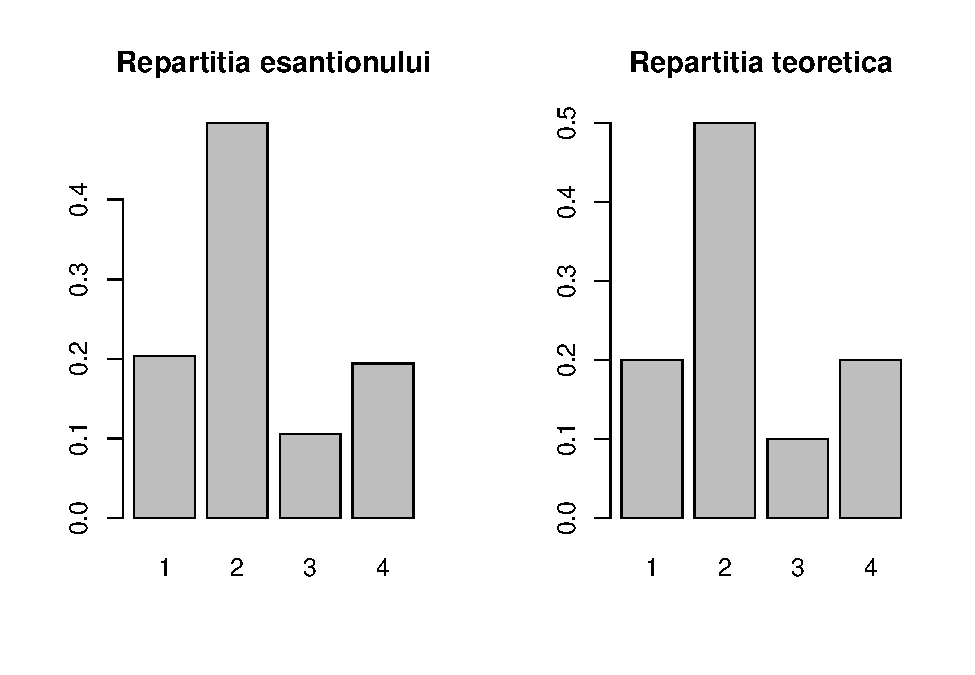
\includegraphics[width=0.8\linewidth]{Lab4_files/figure-latex/unnamed-chunk-7-1} \end{center}

Observăm că eșationul este repartizat conform \(\nu\).

\begin{rmdexercise}
În acest exercițiu ne propunem să definim o funcție
\texttt{rand\_sample(n,x,p)} care permite generarea a \(n\) observații
dintr-o mulțime \(x\) (vector numeric sau de caractere) cu
probabilitatea \(p\) pe \(x\) (un vector de aceeași lungime ca \(x\)).
\end{rmdexercise}

Funcția se poate construi sub forma următoare:

\begin{Shaded}
\begin{Highlighting}[]
\NormalTok{rand_sample =}\StringTok{ }\ControlFlowTok{function}\NormalTok{(n,x,p)\{}
  \CommentTok{# n - numarul de observatii}
  \CommentTok{# x - multimea de valori}
  \CommentTok{# p - vectorul de probabilitati}
  
\NormalTok{  out =}\StringTok{ }\KeywordTok{c}\NormalTok{()}
  
\NormalTok{  ind =}\StringTok{ }\DecValTok{1}\OperatorTok{:}\KeywordTok{length}\NormalTok{(x)}
\NormalTok{  cs =}\StringTok{ }\KeywordTok{cumsum}\NormalTok{(p) }
  
  \ControlFlowTok{if}\NormalTok{ (}\KeywordTok{length}\NormalTok{(x)}\OperatorTok{!=}\KeywordTok{length}\NormalTok{(p))\{}
    \KeywordTok{return}\NormalTok{(}\KeywordTok{print}\NormalTok{(}\StringTok{'Cei doi vectori ar trebui sa fie de aceeasi lungime !'}\NormalTok{))}
\NormalTok{  \}}
  
  \ControlFlowTok{for}\NormalTok{ (i }\ControlFlowTok{in} \DecValTok{1}\OperatorTok{:}\NormalTok{n)\{}
\NormalTok{    r =}\StringTok{ }\KeywordTok{runif}\NormalTok{(}\DecValTok{1}\NormalTok{)}
    
\NormalTok{    m =}\StringTok{ }\KeywordTok{min}\NormalTok{(ind[r}\OperatorTok{<=}\NormalTok{cs])}
\NormalTok{    out =}\StringTok{ }\KeywordTok{c}\NormalTok{(out,x[m])}
\NormalTok{  \}}
  
  \KeywordTok{return}\NormalTok{(out)}
\NormalTok{\}}
\end{Highlighting}
\end{Shaded}

Pentru a testa această funcție să considerăm două exemple:

\begin{enumerate}
\def\labelenumi{\arabic{enumi}.}
\tightlist
\item
  în acest caz: \(n=10\), \(x=[1,2,3]\) și \(p=[0.2,0.3,0.5]\)
\end{enumerate}

\begin{Shaded}
\begin{Highlighting}[]
\KeywordTok{rand_sample}\NormalTok{(}\DecValTok{10}\NormalTok{,}\KeywordTok{c}\NormalTok{(}\DecValTok{1}\NormalTok{,}\DecValTok{2}\NormalTok{,}\DecValTok{3}\NormalTok{),}\KeywordTok{c}\NormalTok{(}\FloatTok{0.2}\NormalTok{,}\FloatTok{0.3}\NormalTok{,}\FloatTok{0.5}\NormalTok{))}
\NormalTok{ [}\DecValTok{1}\NormalTok{] }\DecValTok{3} \DecValTok{2} \DecValTok{3} \DecValTok{3} \DecValTok{1} \DecValTok{1} \DecValTok{1} \DecValTok{3} \DecValTok{1} \DecValTok{3}
\end{Highlighting}
\end{Shaded}

\begin{enumerate}
\def\labelenumi{\arabic{enumi}.}
\setcounter{enumi}{1}
\tightlist
\item
  în acest caz: \(n=15\), \(x=[a,b,c,d]\) și \(p=[0.15,0.35,0.15,0.45]\)
\end{enumerate}

\begin{Shaded}
\begin{Highlighting}[]
\KeywordTok{rand_sample}\NormalTok{(}\DecValTok{15}\NormalTok{,}\KeywordTok{c}\NormalTok{(}\StringTok{'a'}\NormalTok{,}\StringTok{'b'}\NormalTok{,}\StringTok{'c'}\NormalTok{,}\StringTok{'d'}\NormalTok{),}\KeywordTok{c}\NormalTok{(}\FloatTok{0.15}\NormalTok{,}\FloatTok{0.35}\NormalTok{,}\FloatTok{0.15}\NormalTok{,}\FloatTok{0.45}\NormalTok{))}
\NormalTok{ [}\DecValTok{1}\NormalTok{] }\StringTok{"d"} \StringTok{"d"} \StringTok{"d"} \StringTok{"d"} \StringTok{"a"} \StringTok{"a"} \StringTok{"d"} \StringTok{"c"} \StringTok{"b"} \StringTok{"a"} \StringTok{"a"} \StringTok{"c"} \StringTok{"d"} \StringTok{"a"} \StringTok{"b"}
\end{Highlighting}
\end{Shaded}

O funcție un pic mai generală este:

\begin{Shaded}
\begin{Highlighting}[]
\NormalTok{GenerateDiscrete =}\StringTok{ }\ControlFlowTok{function}\NormalTok{(}\DataTypeTok{n =} \DecValTok{1}\NormalTok{, x, p, }\DataTypeTok{err =} \FloatTok{1e-15}\NormalTok{)\{}
  \CommentTok{# n numarul de observatii}
  \CommentTok{# x multimea de valori}
  \CommentTok{# p vectorul de probabilitati}
  
\NormalTok{  lp =}\StringTok{ }\KeywordTok{length}\NormalTok{(p)}
\NormalTok{  lx =}\StringTok{ }\KeywordTok{length}\NormalTok{(x)}
  
  \CommentTok{# verificarea conditiilor de aplicare }
  \ControlFlowTok{if}\NormalTok{(}\KeywordTok{abs}\NormalTok{(}\KeywordTok{sum}\NormalTok{(p)}\OperatorTok{-}\DecValTok{1}\NormalTok{)}\OperatorTok{>}\NormalTok{err }\OperatorTok{|}\StringTok{ }\KeywordTok{sum}\NormalTok{(p}\OperatorTok{>=}\DecValTok{0}\NormalTok{)}\OperatorTok{!=}\NormalTok{lp)\{}
    
    \KeywordTok{stop}\NormalTok{(}\StringTok{"Suma probabilitatilor nu este egala cu 1!"}\NormalTok{)}
    
\NormalTok{  \}}\ControlFlowTok{else} \ControlFlowTok{if}\NormalTok{(lx}\OperatorTok{!=}\NormalTok{lp)\{}
    
    \KeywordTok{stop}\NormalTok{(}\StringTok{"x si p trebuie sa aiba aceeasi marime!"}\NormalTok{)}
    
\NormalTok{  \}}\ControlFlowTok{else}\NormalTok{\{}
\NormalTok{    out =}\StringTok{ }\KeywordTok{rep}\NormalTok{(}\DecValTok{0}\NormalTok{, n)}
    
\NormalTok{    indOrderProb =}\StringTok{ }\KeywordTok{order}\NormalTok{(p, }\DataTypeTok{decreasing =} \OtherTok{TRUE}\NormalTok{) }\CommentTok{# index}
\NormalTok{    pOrdered =}\StringTok{ }\NormalTok{p[indOrderProb] }\CommentTok{# rearanjam valorile probabilitatilor}
\NormalTok{    xOrdered =}\StringTok{ }\NormalTok{x[indOrderProb] }\CommentTok{# rearanjam valorile lui x}
    
\NormalTok{    pOrderedCS =}\StringTok{ }\KeywordTok{cumsum}\NormalTok{(pOrdered)}
    
    \ControlFlowTok{for}\NormalTok{ (i }\ControlFlowTok{in} \DecValTok{1}\OperatorTok{:}\NormalTok{n)\{}
\NormalTok{      u =}\StringTok{ }\KeywordTok{runif}\NormalTok{(}\DecValTok{1}\NormalTok{)}
      
\NormalTok{      k =}\StringTok{ }\KeywordTok{min}\NormalTok{(}\KeywordTok{which}\NormalTok{(u}\OperatorTok{<=}\NormalTok{pOrderedCS))}
\NormalTok{      out[i] =}\StringTok{ }\NormalTok{xOrdered[k]}
\NormalTok{    \}}
\NormalTok{  \}}
  
  \KeywordTok{return}\NormalTok{(out)}
\NormalTok{\}}
\end{Highlighting}
\end{Shaded}

și pentru a o putea testa să considerăm cazul repartițiilor Poisson și
Geometrică:

\begin{enumerate}
\def\labelenumi{\alph{enumi})}
\tightlist
\item
  Poisson
\end{enumerate}

\begin{Shaded}
\begin{Highlighting}[]
\CommentTok{# Poisson}
\KeywordTok{hist}\NormalTok{(}\KeywordTok{GenerateDiscrete}\NormalTok{(}\DecValTok{10000}\NormalTok{, }\DataTypeTok{x =} \DecValTok{0}\OperatorTok{:}\DecValTok{50}\NormalTok{, }
                      \DataTypeTok{p =} \KeywordTok{dpois}\NormalTok{(}\DecValTok{0}\OperatorTok{:}\DecValTok{50}\NormalTok{, }\DecValTok{5}\NormalTok{)), }
     \DataTypeTok{probability =} \OtherTok{TRUE}\NormalTok{, }
     \DataTypeTok{breaks =} \KeywordTok{seq}\NormalTok{(}\OperatorTok{-}\FloatTok{0.5}\NormalTok{,}\FloatTok{49.5}\NormalTok{, }\DataTypeTok{by =} \DecValTok{1}\NormalTok{), }
     \DataTypeTok{xlim =} \KeywordTok{c}\NormalTok{(}\OperatorTok{-}\FloatTok{0.5}\NormalTok{, }\DecValTok{20}\NormalTok{),}
     \DataTypeTok{col =} \StringTok{"grey80"}\NormalTok{,}
     \DataTypeTok{main =} \StringTok{"Repartitia Poisson"}\NormalTok{,}
     \DataTypeTok{xlab =} \StringTok{"X"}\NormalTok{,}
     \DataTypeTok{ylab =} \StringTok{"Densitatea"}\NormalTok{)}

\KeywordTok{lines}\NormalTok{(}\DecValTok{0}\OperatorTok{:}\DecValTok{50}\NormalTok{,}
      \KeywordTok{dpois}\NormalTok{(}\DecValTok{0}\OperatorTok{:}\DecValTok{50}\NormalTok{, }\DecValTok{5}\NormalTok{), }
      \DataTypeTok{type =} \StringTok{"l"}\NormalTok{, }
      \DataTypeTok{col =}\NormalTok{ myred, }\DataTypeTok{lty =} \DecValTok{2}\NormalTok{, }\DataTypeTok{lwd =} \DecValTok{3}\NormalTok{)}
\end{Highlighting}
\end{Shaded}

\begin{center}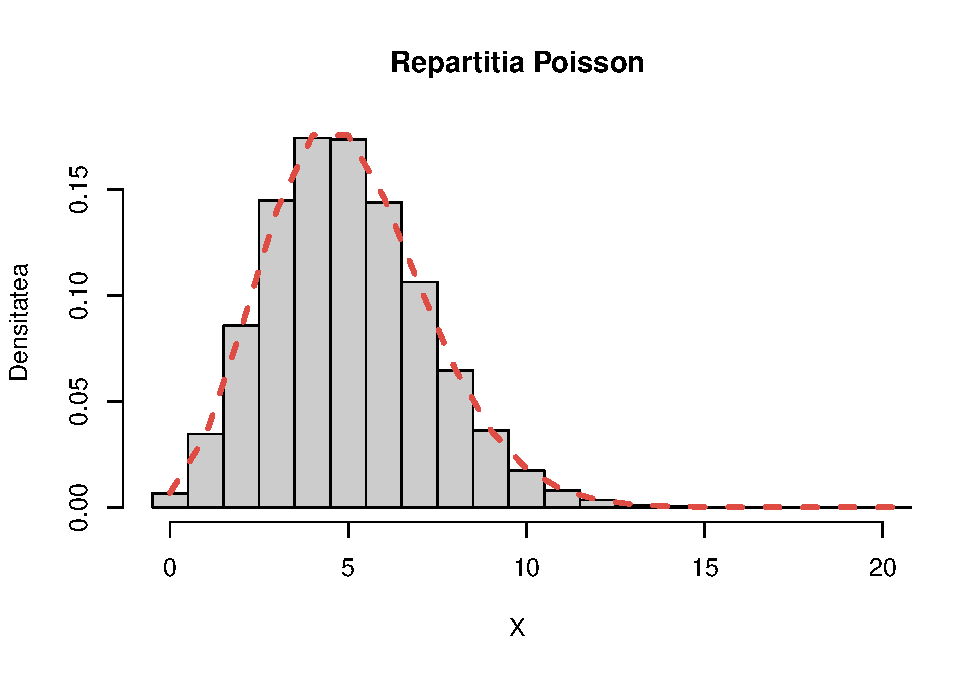
\includegraphics[width=0.8\linewidth]{Lab4_files/figure-latex/unnamed-chunk-13-1} \end{center}

\begin{enumerate}
\def\labelenumi{\alph{enumi})}
\setcounter{enumi}{1}
\tightlist
\item
  Geometrică
\end{enumerate}

\begin{Shaded}
\begin{Highlighting}[]
\CommentTok{# Geometric}
\KeywordTok{hist}\NormalTok{(}\KeywordTok{GenerateDiscrete}\NormalTok{(}\DecValTok{10000}\NormalTok{, }\DataTypeTok{x =} \DecValTok{0}\OperatorTok{:}\DecValTok{100}\NormalTok{, }
                      \DataTypeTok{p =} \KeywordTok{dgeom}\NormalTok{(}\DecValTok{0}\OperatorTok{:}\DecValTok{100}\NormalTok{, }\FloatTok{0.3}\NormalTok{)), }
     \DataTypeTok{probability =} \OtherTok{TRUE}\NormalTok{, }
     \DataTypeTok{breaks =} \KeywordTok{seq}\NormalTok{(}\OperatorTok{-}\FloatTok{0.5}\NormalTok{,}\FloatTok{99.5}\NormalTok{, }\DataTypeTok{by =} \DecValTok{1}\NormalTok{),}
     \DataTypeTok{xlim =} \KeywordTok{c}\NormalTok{(}\OperatorTok{-}\FloatTok{0.5}\NormalTok{, }\DecValTok{20}\NormalTok{),}
     \DataTypeTok{col =} \StringTok{"grey80"}\NormalTok{,}
     \DataTypeTok{main =} \StringTok{"Repartitia Geometrica"}\NormalTok{,}
     \DataTypeTok{xlab =} \StringTok{"X"}\NormalTok{,}
     \DataTypeTok{ylab =} \StringTok{"Densitatea"}\NormalTok{)}

\KeywordTok{lines}\NormalTok{(}\DecValTok{0}\OperatorTok{:}\DecValTok{100}\NormalTok{,}
      \KeywordTok{dgeom}\NormalTok{(}\DecValTok{0}\OperatorTok{:}\DecValTok{100}\NormalTok{, }\FloatTok{0.3}\NormalTok{), }
      \DataTypeTok{type =} \StringTok{"l"}\NormalTok{, }
      \DataTypeTok{col =}\NormalTok{ myred, }\DataTypeTok{lty =} \DecValTok{2}\NormalTok{, }\DataTypeTok{lwd =} \DecValTok{3}\NormalTok{)}
\end{Highlighting}
\end{Shaded}

\begin{center}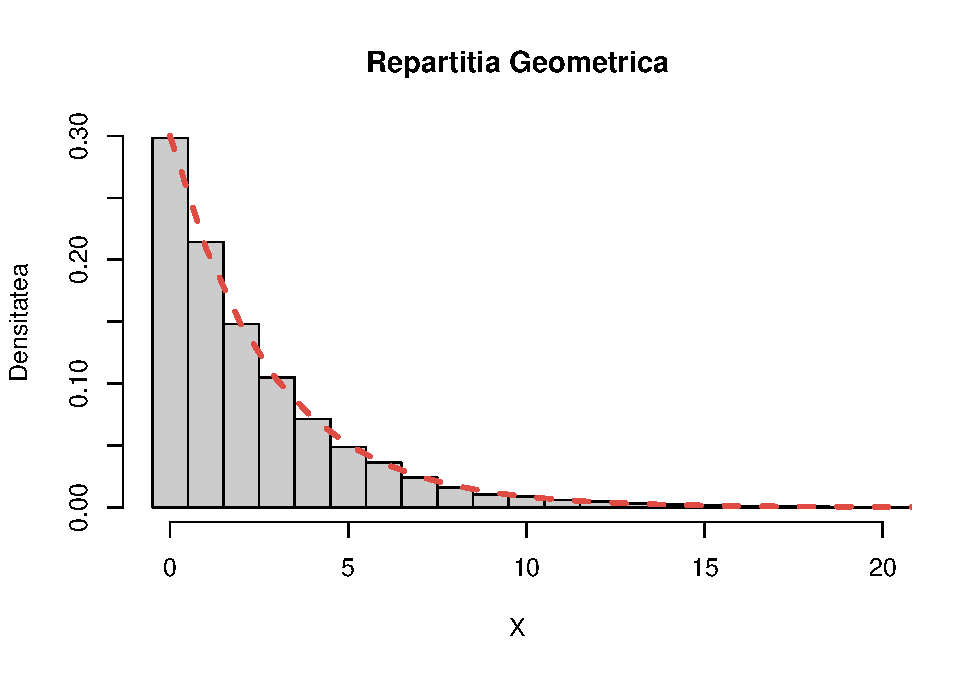
\includegraphics[width=0.8\linewidth]{Lab4_files/figure-latex/unnamed-chunk-14-1} \end{center}

\section{Generarea unei variabile aleatoare folosind metoda
inversă}\label{generarea-unei-variabile-aleatoare-folosind-metoda-inversa}

\begin{rmdexercise}
Scrieți un program care să folosească metoda transformării inverse
pentru a genera \(n\) observații din densitatea

\[
  f(x) = \left\{\begin{array}{ll}
        \frac{1}{x^2}, & x\geq 1\\
        0, & \text{altfel}
  \end{array}\right.
\]

Testați programul trasând o histogramă a \(10000\) de observații
aleatoare împreună cu densitatea teoretică \(f\).
\end{rmdexercise}

Primul pas este să determinăm funcția de repartiție \(F\)
corespunzătoare acestei densități. Pentru \(x<1\) avem că \(f(x)=0\)
deci \(F(x)=0\) iar pentru \(x\geq 1\) avem

\[
  F(x) = \int_{1}^{x}\frac{1}{t^2}\, dt = 1 - \frac{1}{x}.
\]

Cum \(F\) este continuă putem să determinăm \(F^{-1}\) rezolvând ecuația
\(F(x)=u\). Un calcul direct conduce la \(F^{-1}(u)=\frac{1}{1-u}\) iar
conform rezultatului văzut la curs concluzionăm că \(X = \frac{1}{1-U}\)
cu \(U\sim \mathcal{U}([0,1])\).

Astfel putem simula un eșantion de talie \(n\) din populația \(f\)
construind funcția

\begin{Shaded}
\begin{Highlighting}[]
\NormalTok{GenerateSampleX =}\StringTok{ }\ControlFlowTok{function}\NormalTok{(n)\{}
\NormalTok{  u =}\StringTok{ }\KeywordTok{runif}\NormalTok{(n)}
  \KeywordTok{return}\NormalTok{(}\DecValTok{1}\OperatorTok{/}\NormalTok{(}\DecValTok{1}\OperatorTok{-}\NormalTok{u))}
\NormalTok{\}}
\end{Highlighting}
\end{Shaded}

Pentru a testa comparăm valorile simulate cu densitatea teoretică

\begin{Shaded}
\begin{Highlighting}[]
\CommentTok{# simulate}
\NormalTok{x =}\StringTok{ }\KeywordTok{GenerateSampleX}\NormalTok{(}\DecValTok{10000}\NormalTok{)}
\KeywordTok{hist}\NormalTok{(x, }\DataTypeTok{freq=}\OtherTok{FALSE}\NormalTok{, }\DataTypeTok{breaks=}\KeywordTok{seq}\NormalTok{(}\DecValTok{0}\NormalTok{, }\KeywordTok{max}\NormalTok{(x)}\OperatorTok{+}\DecValTok{1}\NormalTok{, }\FloatTok{0.1}\NormalTok{),}
     \DataTypeTok{xlim=}\KeywordTok{c}\NormalTok{(}\DecValTok{0}\NormalTok{,}\DecValTok{10}\NormalTok{), }\DataTypeTok{ylim=}\KeywordTok{c}\NormalTok{(}\DecValTok{0}\NormalTok{,}\DecValTok{1}\NormalTok{),}
     \DataTypeTok{ylab =} \StringTok{"Densitatea"}\NormalTok{,}
     \DataTypeTok{main=}\OtherTok{NULL}\NormalTok{, }\DataTypeTok{col=}\StringTok{"gray80"}\NormalTok{, }\DataTypeTok{border=}\StringTok{"gray20"}\NormalTok{)}

\CommentTok{# densitatea teoretica}
\NormalTok{y =}\StringTok{ }\KeywordTok{seq}\NormalTok{(}\DecValTok{0}\NormalTok{, }\DecValTok{10}\NormalTok{, }\FloatTok{0.01}\NormalTok{)}
\NormalTok{f =}\StringTok{ }\KeywordTok{ifelse}\NormalTok{(y }\OperatorTok{<=}\StringTok{ }\DecValTok{1}\NormalTok{, }\DecValTok{0}\NormalTok{, }\DecValTok{1}\OperatorTok{/}\NormalTok{y}\OperatorTok{^}\DecValTok{2}\NormalTok{)}
\KeywordTok{lines}\NormalTok{(y, f, }\DataTypeTok{col =}\NormalTok{ myred, }\DataTypeTok{lty =} \DecValTok{2}\NormalTok{, }\DataTypeTok{lwd =} \DecValTok{3}\NormalTok{)}
\end{Highlighting}
\end{Shaded}

\begin{center}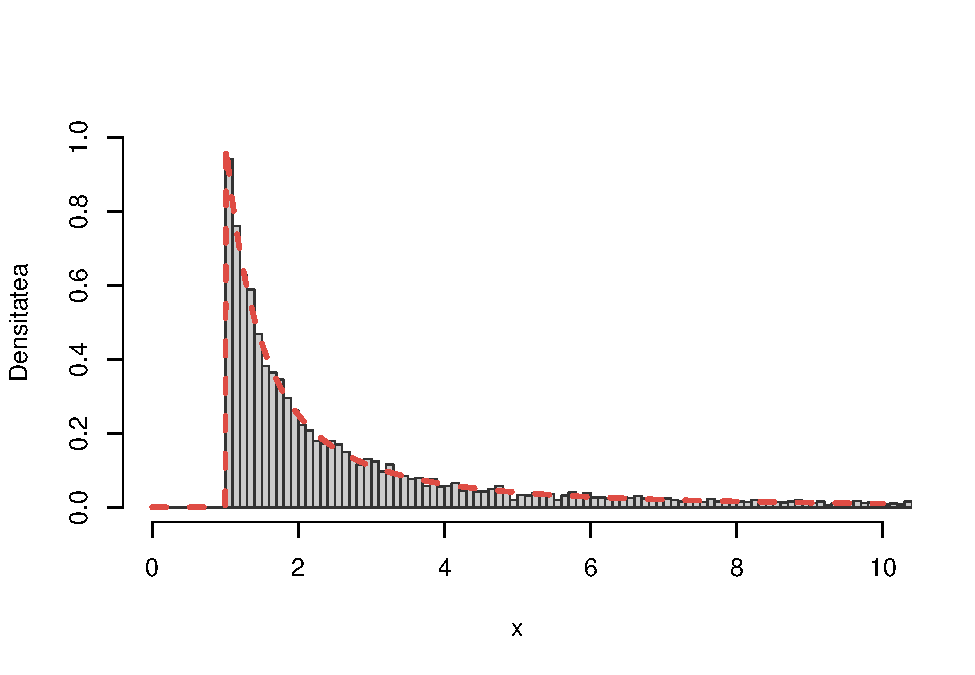
\includegraphics[width=0.8\linewidth]{Lab4_files/figure-latex/unnamed-chunk-17-1} \end{center}

\begin{rmdexercise}
\begin{enumerate}
\def\labelenumi{\arabic{enumi}.}
\item
  Folosind metoda inversă, simulați \(10000\) de observații independente
  din repartiția \(\mathcal{E}(\lambda)\), cu \(\lambda = 1\). Trasați
  histograma acestui eșantion și comparați cu densitatea repartiției.
\item
  Fie \(X_1, \ldots, X_n\), \(n\) variabile aleatoare i.i.d. repartizate
  \(\mathcal{E}(\lambda)\). Atunci variabila aleatoare
  \(S_n = X_1 + X_2 +\cdots+ X_n\) este repartizată
  \(\Gamma(n, \lambda)\). Plecând de la acest rezultat, generați
  \(10000\) de observații din repartiția \(\Gamma(n, \lambda)\)
  (\(n = 10\)). Trasați histograma acestui eșantion și comparați cu
  densitatea legii.
\item
  Dacă definim \(N = \sup\{n\geq 1\,|\, S_n\leq 1\}\) (folosim convenția
  \(N = 0\) dacă \(S_1>1\)), atunci \(N\) este repartizată Poisson
  \(Pois(\lambda)\). Plecând de la acest rezultat, generați \(10000\) de
  observații independente din repartiția \(Pois(\lambda)\), trasați
  histograma acestui eșantion și comparați cu repartiția teoretică.
\end{enumerate}
\end{rmdexercise}

\begin{enumerate}
\def\labelenumi{\arabic{enumi}.}
\tightlist
\item
  Metoda funcției inverse conduce la
  \(-\frac{\log(U)}{\lambda}\sim\mathcal{E}(\lambda)\), cu
  \(U\sim\mathcal{U}([0,1])\).
\end{enumerate}

\begin{Shaded}
\begin{Highlighting}[]
\NormalTok{sim.exp =}\StringTok{ }\ControlFlowTok{function}\NormalTok{(n, }\DataTypeTok{lambda =} \DecValTok{1}\NormalTok{)\{}
  \KeywordTok{return}\NormalTok{(}\OperatorTok{-}\KeywordTok{log}\NormalTok{(}\KeywordTok{runif}\NormalTok{(n))}\OperatorTok{/}\NormalTok{lambda)}
\NormalTok{\}}

\NormalTok{n =}\StringTok{ }\DecValTok{10000}

\NormalTok{x =}\StringTok{ }\KeywordTok{sim.exp}\NormalTok{(n)}
\end{Highlighting}
\end{Shaded}

Pentru trasarea histogramei avem:

\begin{Shaded}
\begin{Highlighting}[]
\KeywordTok{hist}\NormalTok{(x, }\DataTypeTok{freq =} \OtherTok{FALSE}\NormalTok{, }
     \DataTypeTok{col=}\StringTok{"gray80"}\NormalTok{, }
     \DataTypeTok{border=}\StringTok{"gray20"}\NormalTok{,}
     \DataTypeTok{main =} \StringTok{"Histograma lui x"}\NormalTok{, }
     \DataTypeTok{ylab =} \StringTok{""}\NormalTok{, }\DataTypeTok{xlab =} \StringTok{""}\NormalTok{)}

\NormalTok{t =}\StringTok{ }\KeywordTok{seq}\NormalTok{(}\DecValTok{0}\NormalTok{, }\KeywordTok{max}\NormalTok{(x), }\FloatTok{0.01}\NormalTok{)}
\KeywordTok{lines}\NormalTok{(t, }\KeywordTok{dexp}\NormalTok{(t), }
      \DataTypeTok{col =}\NormalTok{ myred, }
      \DataTypeTok{lty =} \DecValTok{2}\NormalTok{, }\DataTypeTok{lwd =} \DecValTok{3}\NormalTok{)}
\KeywordTok{legend}\NormalTok{(}\StringTok{"topright"}\NormalTok{, }
       \StringTok{"Densitatea exponentialei"}\NormalTok{, }
       \DataTypeTok{box.lty =} \DecValTok{0}\NormalTok{,}
       \DataTypeTok{col =}\NormalTok{ myred, }
       \DataTypeTok{lty =} \DecValTok{2}\NormalTok{, }\DataTypeTok{lwd =} \DecValTok{3}\NormalTok{, }\DataTypeTok{inset =} \FloatTok{0.05}\NormalTok{)}
\end{Highlighting}
\end{Shaded}

\begin{center}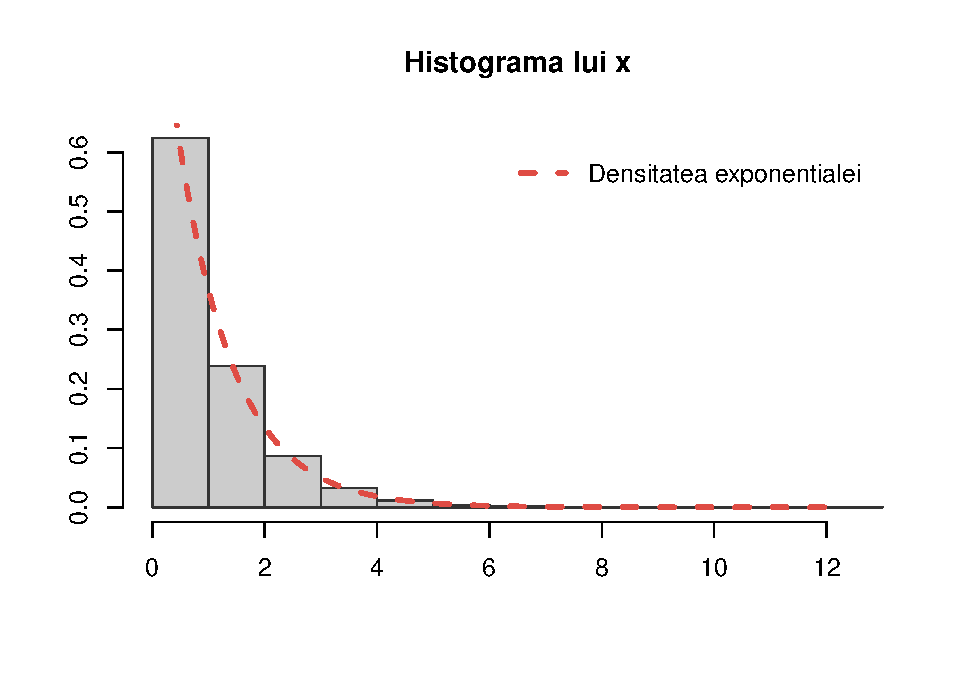
\includegraphics[width=0.8\linewidth]{Lab4_files/figure-latex/unnamed-chunk-20-1} \end{center}

Să observăm că în R putem folosi funcția \texttt{rexp(n,\ rate\ =\ ...)}
pentru generarea de observații repartizate exponențial.

\begin{enumerate}
\def\labelenumi{\arabic{enumi}.}
\setcounter{enumi}{1}
\tightlist
\item
  Pentru generarea a \(m\) variabile aleatoare i.i.d. repartizate
  \(\Gamma(n, \lambda)\), simulăm \(m\times n\) variabile repartizate
  exponențial pe care le stocăm într-o matrice cu \(m\) linii și \(n\)
  coloane. Suma elementelor de pe o linie reprezintă o realizate a
  repartiției \(\Gamma(n, \lambda)\).
\end{enumerate}

\begin{Shaded}
\begin{Highlighting}[]
\NormalTok{sim.gamma =}\StringTok{ }\ControlFlowTok{function}\NormalTok{(m, n, }\DataTypeTok{lambda =} \DecValTok{1}\NormalTok{)\{}
\NormalTok{  out =}\StringTok{ }\KeywordTok{rowSums}\NormalTok{(}\KeywordTok{matrix}\NormalTok{(}\KeywordTok{sim.exp}\NormalTok{(m }\OperatorTok{*}\StringTok{ }\NormalTok{n, lambda), m, n))}
  \KeywordTok{return}\NormalTok{(out)}
\NormalTok{\}}
\end{Highlighting}
\end{Shaded}

Din punct de vedere al costului de memorie, această metodă poate să nu
fie optimă. Putem folosi o abordare mai simplă folosind bucla
\texttt{for}:

\begin{Shaded}
\begin{Highlighting}[]
\NormalTok{sim.gamma2 =}\StringTok{ }\ControlFlowTok{function}\NormalTok{(m, n, }\DataTypeTok{lambda =} \DecValTok{1}\NormalTok{)\{}
\NormalTok{  out =}\StringTok{ }\KeywordTok{numeric}\NormalTok{(m)}
  
  \ControlFlowTok{for}\NormalTok{ (i }\ControlFlowTok{in} \DecValTok{1}\OperatorTok{:}\NormalTok{m)\{}
\NormalTok{    out[i] =}\StringTok{ }\KeywordTok{sum}\NormalTok{(}\KeywordTok{sim.exp}\NormalTok{(n, lambda))}
\NormalTok{  \}}
  
  \KeywordTok{return}\NormalTok{(out)}
\NormalTok{\}}
\end{Highlighting}
\end{Shaded}

Pentru verificare avem

\begin{Shaded}
\begin{Highlighting}[]
\NormalTok{n =}\StringTok{ }\DecValTok{10}
\NormalTok{m =}\StringTok{ }\DecValTok{10000}

\NormalTok{x =}\StringTok{ }\KeywordTok{sim.gamma}\NormalTok{(m, n)}
\NormalTok{t =}\StringTok{ }\KeywordTok{seq}\NormalTok{(}\KeywordTok{min}\NormalTok{(x), }\KeywordTok{max}\NormalTok{(x), }\FloatTok{0.01}\NormalTok{)}

\KeywordTok{hist}\NormalTok{(x, }\DataTypeTok{freq =} \OtherTok{FALSE}\NormalTok{, }
     \DataTypeTok{col=}\StringTok{"gray80"}\NormalTok{, }
     \DataTypeTok{border=}\StringTok{"gray20"}\NormalTok{,}
     \DataTypeTok{main =} \StringTok{"Histograma lui x"}\NormalTok{, }\DataTypeTok{ylab =} \StringTok{""}\NormalTok{, }
     \DataTypeTok{xlab =} \StringTok{""}\NormalTok{)}

\KeywordTok{lines}\NormalTok{(t, }\KeywordTok{dgamma}\NormalTok{(t, n), }
      \DataTypeTok{col =}\NormalTok{ myred, }\DataTypeTok{lwd =} \DecValTok{3}\NormalTok{, }\DataTypeTok{lty =} \DecValTok{2}\NormalTok{)}
\KeywordTok{legend}\NormalTok{(}\StringTok{"topright"}\NormalTok{, }
       \StringTok{"Densitatea rep. gamma"}\NormalTok{, }
       \DataTypeTok{box.lty =} \DecValTok{0}\NormalTok{,}
       \DataTypeTok{col =}\NormalTok{ myred, }
       \DataTypeTok{lty =} \DecValTok{2}\NormalTok{, }\DataTypeTok{lwd =} \DecValTok{3}\NormalTok{, }\DataTypeTok{inset =} \FloatTok{0.05}\NormalTok{)}
\end{Highlighting}
\end{Shaded}

\begin{center}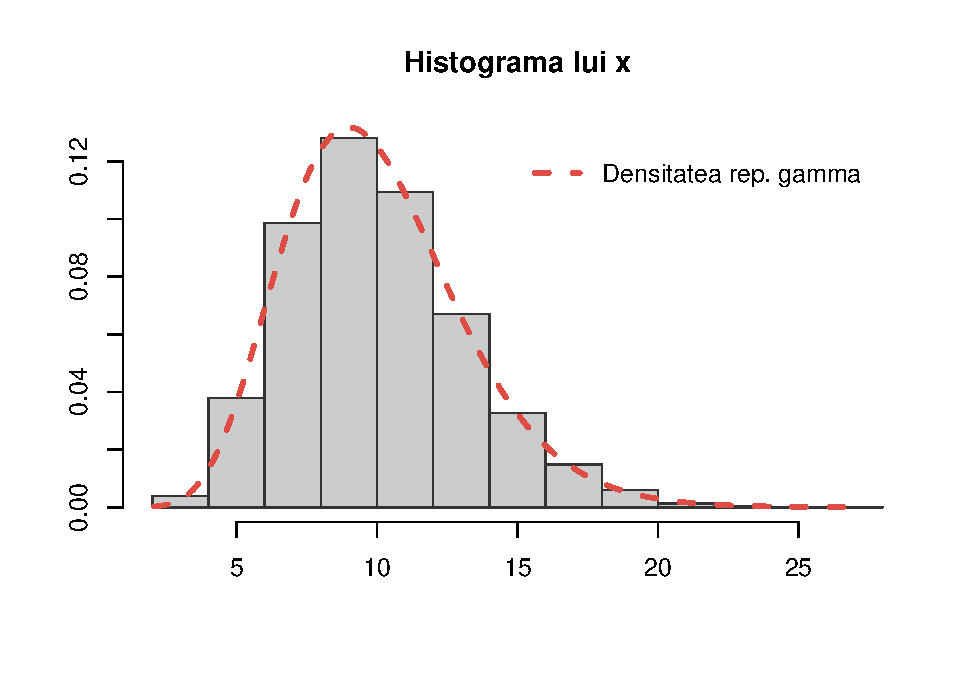
\includegraphics[width=0.8\linewidth]{Lab4_files/figure-latex/unnamed-chunk-23-1} \end{center}

\begin{enumerate}
\def\labelenumi{\arabic{enumi}.}
\setcounter{enumi}{2}
\tightlist
\item
  Umătoarea funcție generează observații repartizate Poisson conform
  enunțului:
\end{enumerate}

\begin{Shaded}
\begin{Highlighting}[]
\NormalTok{sim.pois1 =}\StringTok{ }\ControlFlowTok{function}\NormalTok{(n, }\DataTypeTok{lambda =} \DecValTok{1}\NormalTok{)\{}
\NormalTok{  out =}\StringTok{ }\KeywordTok{numeric}\NormalTok{(n)}
  
  \ControlFlowTok{for}\NormalTok{ (i }\ControlFlowTok{in} \DecValTok{1}\OperatorTok{:}\NormalTok{n)\{}
\NormalTok{    out[i] =}\StringTok{ }\DecValTok{0}
\NormalTok{    s =}\StringTok{ }\OperatorTok{-}\KeywordTok{log}\NormalTok{(}\KeywordTok{runif}\NormalTok{(}\DecValTok{1}\NormalTok{))}\OperatorTok{/}\NormalTok{lambda}
    \ControlFlowTok{while}\NormalTok{(s}\OperatorTok{<=}\DecValTok{1}\NormalTok{)\{}
\NormalTok{      s =}\StringTok{ }\NormalTok{s }\OperatorTok{-}\StringTok{ }\KeywordTok{log}\NormalTok{(}\KeywordTok{runif}\NormalTok{(}\DecValTok{1}\NormalTok{))}\OperatorTok{/}\NormalTok{lambda }
\NormalTok{      out[i] =}\StringTok{ }\NormalTok{out[i] }\OperatorTok{+}\StringTok{ }\DecValTok{1}
\NormalTok{    \}}
\NormalTok{  \}}
  
  \KeywordTok{return}\NormalTok{(out)}
\NormalTok{\}}
\end{Highlighting}
\end{Shaded}

Această funcție ar putea fi costisitoare în ceea ce privește timpul de
execuție (R nu este foarte eficient atunci când avem bucle imbricate).
Avem următoare funcție:

\begin{Shaded}
\begin{Highlighting}[]
\NormalTok{sim.pois2 =}\StringTok{ }\ControlFlowTok{function}\NormalTok{(n, }\DataTypeTok{lambda =} \DecValTok{1}\NormalTok{)\{}
\NormalTok{  x =}\StringTok{ }\KeywordTok{sim.exp}\NormalTok{(n, lambda)}
\NormalTok{  i =}\StringTok{ }\DecValTok{0}
\NormalTok{  l =}\StringTok{ }\KeywordTok{which}\NormalTok{(x}\OperatorTok{<=}\DecValTok{1}\NormalTok{)}
  \CommentTok{# realizari cu valoarea 0}
\NormalTok{  out =}\StringTok{ }\KeywordTok{rep}\NormalTok{(}\DecValTok{0}\NormalTok{, }\KeywordTok{sum}\NormalTok{(x }\OperatorTok{>}\StringTok{ }\DecValTok{1}\NormalTok{)) }
  
  \ControlFlowTok{while}\NormalTok{(}\KeywordTok{length}\NormalTok{(l) }\OperatorTok{>}\StringTok{ }\DecValTok{0}\NormalTok{)\{}
\NormalTok{    i =}\StringTok{ }\NormalTok{i }\OperatorTok{+}\StringTok{ }\DecValTok{1}
\NormalTok{    x =}\StringTok{ }\NormalTok{x[l] }\OperatorTok{+}\StringTok{ }\KeywordTok{sim.exp}\NormalTok{(}\KeywordTok{length}\NormalTok{(l), lambda)}
\NormalTok{    l =}\StringTok{ }\KeywordTok{which}\NormalTok{(x}\OperatorTok{<=}\DecValTok{1}\NormalTok{)}
    \CommentTok{# realizari cu valoarea i}
\NormalTok{    out =}\StringTok{ }\KeywordTok{c}\NormalTok{(out, }\KeywordTok{rep}\NormalTok{(i, }\KeywordTok{sum}\NormalTok{(x }\OperatorTok{>}\StringTok{ }\DecValTok{1}\NormalTok{))) }
\NormalTok{  \}}
  
  \KeywordTok{return}\NormalTok{(out)}
\NormalTok{\}}
\end{Highlighting}
\end{Shaded}

Pentru a compara cele două funcții:

\begin{Shaded}
\begin{Highlighting}[]
\NormalTok{n =}\StringTok{ }\DecValTok{100000}

\NormalTok{start =}\StringTok{ }\KeywordTok{proc.time}\NormalTok{()}
\NormalTok{y =}\StringTok{ }\KeywordTok{sim.pois1}\NormalTok{(n)}
\KeywordTok{proc.time}\NormalTok{() }\OperatorTok{-}\StringTok{ }\NormalTok{start}
\NormalTok{   user  system elapsed }
   \FloatTok{0.32}    \FloatTok{0.00}    \FloatTok{0.31} 

\NormalTok{start =}\StringTok{ }\KeywordTok{proc.time}\NormalTok{()}
\NormalTok{x =}\StringTok{ }\KeywordTok{sim.pois2}\NormalTok{(n)}
\KeywordTok{proc.time}\NormalTok{() }\OperatorTok{-}\StringTok{ }\NormalTok{start}
\NormalTok{   user  system elapsed }
   \FloatTok{0.03}    \FloatTok{0.00}    \FloatTok{0.03} 
\end{Highlighting}
\end{Shaded}

Eșantionul generat este repartizat conform repartiției Poisson de
parametru \(\lambda\):

\begin{Shaded}
\begin{Highlighting}[]
\NormalTok{x.freq =}\StringTok{ }\KeywordTok{table}\NormalTok{(x)}\OperatorTok{/}\NormalTok{n}

\KeywordTok{par}\NormalTok{(}\DataTypeTok{mfrow =} \KeywordTok{c}\NormalTok{(}\DecValTok{1}\NormalTok{,}\DecValTok{2}\NormalTok{))}

\KeywordTok{barplot}\NormalTok{(x.freq, }
        \DataTypeTok{main =} \StringTok{"Repartitia esantionului"}\NormalTok{)}

\KeywordTok{barplot}\NormalTok{(}\KeywordTok{dpois}\NormalTok{(}\DecValTok{0}\OperatorTok{:}\KeywordTok{max}\NormalTok{(x), }\DecValTok{1}\NormalTok{), }\DataTypeTok{names.arg =} \DecValTok{0}\OperatorTok{:}\KeywordTok{max}\NormalTok{(x), }
        \DataTypeTok{main =} \StringTok{"Repartitia teoretica"}\NormalTok{)}
\end{Highlighting}
\end{Shaded}

\begin{center}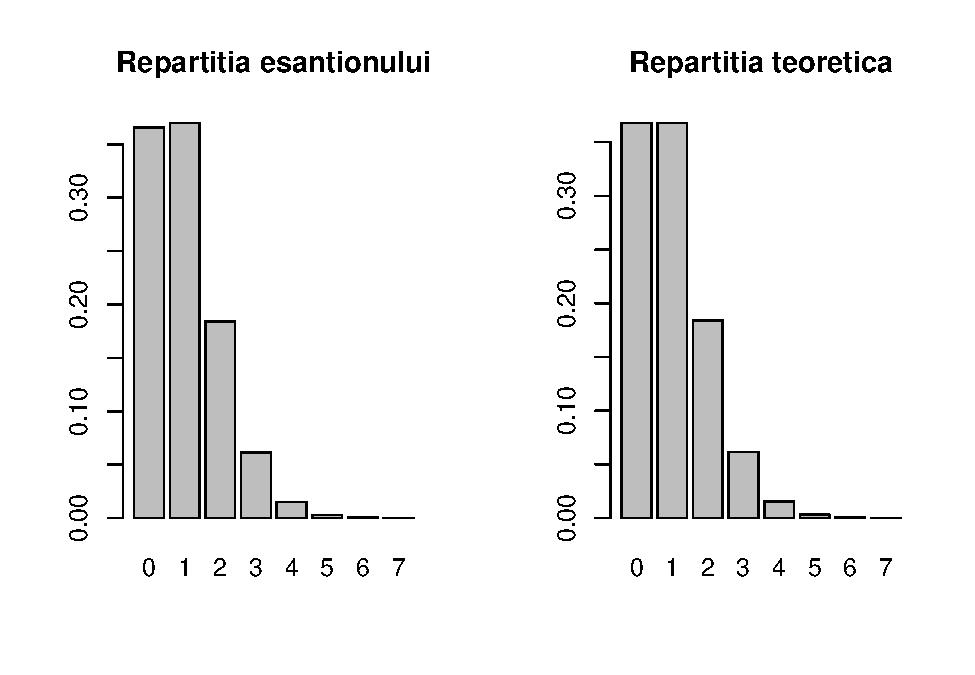
\includegraphics[width=0.8\linewidth]{Lab4_files/figure-latex/unnamed-chunk-27-1} \end{center}

\section{Generarea unei variabile aleatoare folosind metoda
respingerii}\label{generarea-unei-variabile-aleatoare-folosind-metoda-respingerii}

\begin{rmdexercise}
Fie \(f\) densitatea de repartiție definită prin

\[
  f(x) = \frac{2}{\pi}\sqrt{1-x^2}\mathbf{1}_{[-1,1]}(x)
\]

\begin{enumerate}
\def\labelenumi{\arabic{enumi}.}
\item
  Folosiți metoda respingerii pentru a genera \(10000\) de observații
  repartizate cu densitatea \(f\).
\item
  Trasați histograma acestui eșantion și comparați cu densitatea \(f\).
\end{enumerate}
\end{rmdexercise}

\begin{enumerate}
\def\labelenumi{\arabic{enumi}.}
\tightlist
\item
  Observăm că
\end{enumerate}

\[
  f(x) \leq \frac{2}{\pi}\mathbf{1}_{[-1,1]}(x) = \frac{4}{\pi}g(x)
\]

unde \(g(x) = \frac{1}{2}\mathbf{1}_{[-1,1]}(x)\) este densitatea
repartiției uniforme pe \([-1,1]\). Astfel metoda respingerii sugerează
următorul algoritm:

\begin{Shaded}
\begin{Highlighting}[]
\NormalTok{f =}\StringTok{ }\ControlFlowTok{function}\NormalTok{(x)\{}
  \KeywordTok{return}\NormalTok{(}\DecValTok{2}\OperatorTok{/}\NormalTok{pi }\OperatorTok{*}\StringTok{ }\KeywordTok{sqrt}\NormalTok{(}\DecValTok{1}\OperatorTok{-}\NormalTok{x}\OperatorTok{^}\DecValTok{2}\NormalTok{)}\OperatorTok{*}\NormalTok{(}\KeywordTok{abs}\NormalTok{(x) }\OperatorTok{<=}\StringTok{ }\DecValTok{1}\NormalTok{))}
\NormalTok{\}}

\NormalTok{sim.resp1 =}\StringTok{ }\ControlFlowTok{function}\NormalTok{(n)\{}
\NormalTok{  x =}\StringTok{ }\KeywordTok{rep}\NormalTok{(}\DecValTok{0}\NormalTok{, n)}
  
  \ControlFlowTok{for}\NormalTok{ (i }\ControlFlowTok{in} \DecValTok{1}\OperatorTok{:}\NormalTok{n)\{}
    \CommentTok{# generam obs din g}
\NormalTok{    x[i] =}\StringTok{ }\KeywordTok{runif}\NormalTok{(}\DecValTok{1}\NormalTok{, }\OperatorTok{-}\DecValTok{1}\NormalTok{, }\DecValTok{1}\NormalTok{)}
    
    \CommentTok{# generam uniforma}
\NormalTok{    u =}\StringTok{ }\KeywordTok{runif}\NormalTok{(}\DecValTok{1}\NormalTok{)}
    
    \ControlFlowTok{while}\NormalTok{(u }\OperatorTok{>}\StringTok{ }\NormalTok{pi }\OperatorTok{*}\StringTok{ }\KeywordTok{f}\NormalTok{(x[i])}\OperatorTok{/}\DecValTok{2}\NormalTok{)\{}
\NormalTok{      x[i] =}\StringTok{ }\KeywordTok{runif}\NormalTok{(}\DecValTok{1}\NormalTok{, }\OperatorTok{-}\DecValTok{1}\NormalTok{, }\DecValTok{1}\NormalTok{)    }
\NormalTok{      u =}\StringTok{ }\KeywordTok{runif}\NormalTok{(}\DecValTok{1}\NormalTok{)}
\NormalTok{    \}}
\NormalTok{  \}}
  
  \KeywordTok{return}\NormalTok{(x)}
\NormalTok{\}}
\end{Highlighting}
\end{Shaded}

Putem îmbunătății codul de mai sus (vrem să evităm să avem și bucla
\texttt{for} și bucla \texttt{while} imbricate) dacă ținem cont de
faptul că probabilitatea de acceptare este \(p = \frac{\pi}{4}\) iar
pentru a genera un eșantion de \(m\) observații avem nevoie, în medie,
de \(\frac{m}{p}\) simulări. Avem

\begin{Shaded}
\begin{Highlighting}[]
\NormalTok{sim.resp2 =}\StringTok{ }\ControlFlowTok{function}\NormalTok{(n)\{}
\NormalTok{  out =}\StringTok{ }\KeywordTok{c}\NormalTok{() }\CommentTok{# esantionul final}
  
  \CommentTok{# cate obs mai avem de generat}
\NormalTok{  m =}\StringTok{ }\NormalTok{n}
  
  \CommentTok{# cat timp nu avem esantionul de talia dorita }
  \CommentTok{# continuam procedeul }
  \ControlFlowTok{while}\NormalTok{ (m}\OperatorTok{>}\DecValTok{0}\NormalTok{)\{}
    \CommentTok{# simulam m/p observatii}
\NormalTok{    x =}\StringTok{ }\KeywordTok{runif}\NormalTok{((}\DecValTok{4}\OperatorTok{*}\NormalTok{m)}\OperatorTok\NormalTok{pi }\OperatorTok{+}\StringTok{ }\DecValTok{1}\NormalTok{, }\OperatorTok{-}\DecValTok{1}\NormalTok{, }\DecValTok{1}\NormalTok{)}
\NormalTok{    u =}\StringTok{ }\KeywordTok{runif}\NormalTok{((}\DecValTok{4}\OperatorTok{*}\NormalTok{m)}\OperatorTok\NormalTok{pi }\OperatorTok{+}\StringTok{ }\DecValTok{1}\NormalTok{)}
    
    \CommentTok{# testam care obs sunt acceptate}
\NormalTok{    y =}\StringTok{ }\NormalTok{(u }\OperatorTok{<=}\StringTok{ }\NormalTok{pi }\OperatorTok{*}\StringTok{ }\KeywordTok{f}\NormalTok{(x)}\OperatorTok{/}\DecValTok{2}\NormalTok{)}
    
    \CommentTok{# pastram doar punctele acceptate}
\NormalTok{    out =}\StringTok{ }\KeywordTok{c}\NormalTok{(out, x[}\KeywordTok{which}\NormalTok{(y)])}
\NormalTok{    m =}\StringTok{ }\NormalTok{n }\OperatorTok{-}\StringTok{ }\KeywordTok{length}\NormalTok{(out)}
\NormalTok{  \}}
  
  \KeywordTok{return}\NormalTok{(out[}\DecValTok{1}\OperatorTok{:}\NormalTok{n])}
\NormalTok{\}}
\end{Highlighting}
\end{Shaded}

Putem compara cele două metode, în funcție de timpul de execuție:

\begin{Shaded}
\begin{Highlighting}[]
\NormalTok{n =}\StringTok{ }\DecValTok{10000}

\CommentTok{# Metoda 1}
\NormalTok{star =}\StringTok{ }\KeywordTok{proc.time}\NormalTok{()}
\NormalTok{x =}\StringTok{ }\KeywordTok{sim.resp1}\NormalTok{(n)}
\KeywordTok{proc.time}\NormalTok{() }\OperatorTok{-}\StringTok{ }\NormalTok{start}
\NormalTok{   user  system elapsed }
   \FloatTok{0.18}    \FloatTok{0.00}    \FloatTok{0.22} 

\CommentTok{# Metoda 2}
\NormalTok{star =}\StringTok{ }\KeywordTok{proc.time}\NormalTok{()}
\NormalTok{x =}\StringTok{ }\KeywordTok{sim.resp2}\NormalTok{(n)}
\KeywordTok{proc.time}\NormalTok{() }\OperatorTok{-}\StringTok{ }\NormalTok{start}
\NormalTok{   user  system elapsed }
   \FloatTok{0.20}    \FloatTok{0.00}    \FloatTok{0.24} 
\end{Highlighting}
\end{Shaded}

\begin{enumerate}
\def\labelenumi{\arabic{enumi}.}
\setcounter{enumi}{1}
\tightlist
\item
  Putem valida algoritmul propus prin metoda respingerii trasând
  histograma eșantionului:
\end{enumerate}

\begin{Shaded}
\begin{Highlighting}[]
\KeywordTok{hist}\NormalTok{(x, }\DataTypeTok{freq =} \OtherTok{FALSE}\NormalTok{, }
     \DataTypeTok{col=}\StringTok{"gray80"}\NormalTok{, }
     \DataTypeTok{border=}\StringTok{"gray20"}\NormalTok{,}
     \DataTypeTok{main =} \StringTok{"Histograma lui x"}\NormalTok{, }\DataTypeTok{ylab =} \StringTok{""}\NormalTok{, }
     \DataTypeTok{xlab =} \StringTok{""}\NormalTok{)}

\NormalTok{t =}\StringTok{ }\KeywordTok{seq}\NormalTok{(}\OperatorTok{-}\DecValTok{1}\NormalTok{, }\DecValTok{1}\NormalTok{, }\FloatTok{0.01}\NormalTok{)}
\KeywordTok{lines}\NormalTok{(t, }\KeywordTok{f}\NormalTok{(t), }
      \DataTypeTok{col =}\NormalTok{ myred, }\DataTypeTok{lwd =} \DecValTok{3}\NormalTok{, }\DataTypeTok{lty =} \DecValTok{2}\NormalTok{)}
\KeywordTok{legend}\NormalTok{(}\StringTok{"topright"}\NormalTok{, }
       \StringTok{"f(x)"}\NormalTok{, }
       \DataTypeTok{box.lty =} \DecValTok{0}\NormalTok{,}
       \DataTypeTok{col =}\NormalTok{ myred, }
       \DataTypeTok{lty =} \DecValTok{2}\NormalTok{, }\DataTypeTok{lwd =} \DecValTok{3}\NormalTok{, }\DataTypeTok{inset =} \FloatTok{0.05}\NormalTok{)}
\end{Highlighting}
\end{Shaded}

\begin{center}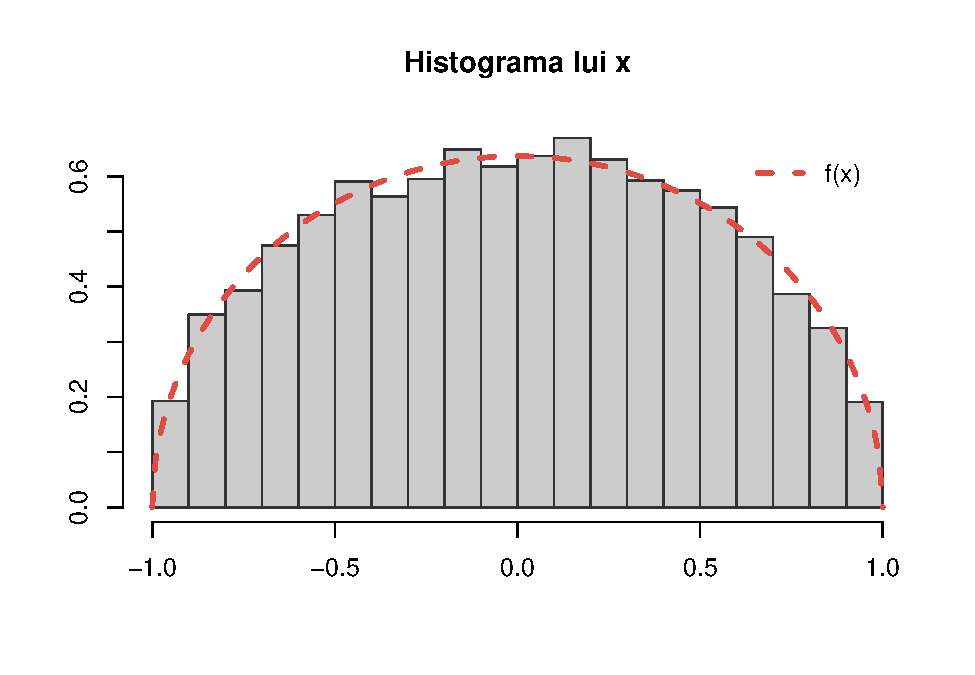
\includegraphics[width=0.8\linewidth]{Lab4_files/figure-latex/unnamed-chunk-32-1} \end{center}

\begin{rmdexercise}
Plecând cu o propunere de tip \(Exp(\lambda)\) vrem să generăm, cu
ajutorul metodei acceptării-respingerii, un eșantion din următoarea
densitate (jumătate de normală):

\[
  f(x) = \left\{\begin{array}{ll}
    \frac{2}{\sqrt{2\pi}}e^{-\frac{x^2}{2}}, & \mbox{dacă $x\geq0$}\\
    0, & \mbox{altfel}\\           
  \end{array}\right.
\]
\end{rmdexercise}

Fie \(g\) densitatea repartiției exponențiale de parametru \(\lambda\),

\[
    g(x) = \left\{\begin{array}{ll}
        \lambda e^{-\lambda x}, & \mbox{dacă $x\geq0$}\\
        0, & \mbox{altfel}\\           
  \end{array}\right.
\]

Pentru a aplica algoritmul de acceptare-respingere trebuie să găsim
valoarea lui \(c>0\) pentru care \(f(x)\leq c g(x)\) pentru toate
valorile \(x\in \mathbb{R}\). Pentru \(x\geq0\) avem

\[
  \frac{f(x)}{g(x)}=\frac{2}{\lambda\sqrt{2\pi}}e^{-\frac{x^2}{2}+\lambda x}
\]

și cum funcția \(-\frac{x^2}{2}+\lambda x\) își atinge valoarea maximă
în punctul \(x=\lambda\) rezultă că

\[
    \frac{f(x)}{g(x)}\leq c^*, \,\,\forall x \geq0
\]

unde

\[
  c^*=\sqrt{\frac{2}{\pi\lambda^2}}e^{\lambda^2/2}.
\]

Astfel algoritmul devine:

\begin{itemize}
\item
  pentru \(n=1,2,\dots\)
\item
  generează \(X_n\sim Exp(\lambda)\)
\item
  generează \(U_n\sim\mathcal{U}[0,1]\)
\item
  dacă \(U_n\leq\exp\left(-\frac{1}{2}(X_n-\lambda)^2\right)\) atunci
\item
  intoarceți \(X_n\)
\end{itemize}

Avem funcția:

\begin{Shaded}
\begin{Highlighting}[]
\CommentTok{# generarea puntelor din densitatea f}

\NormalTok{f <-}\StringTok{ }\ControlFlowTok{function}\NormalTok{(x) \{}
  \KeywordTok{return}\NormalTok{((x}\OperatorTok{>}\StringTok{ }\DecValTok{0}\NormalTok{) }\OperatorTok{*}\StringTok{ }\DecValTok{2} \OperatorTok{*}\StringTok{ }\KeywordTok{dnorm}\NormalTok{(x,}\DecValTok{0}\NormalTok{,}\DecValTok{1}\NormalTok{))}
\NormalTok{\}}

\NormalTok{g <-}\StringTok{ }\ControlFlowTok{function}\NormalTok{(x) \{ }\KeywordTok{return}\NormalTok{(}\KeywordTok{dexp}\NormalTok{(x,}\DecValTok{1}\NormalTok{)) \}}

\NormalTok{c <-}\StringTok{ }\KeywordTok{sqrt}\NormalTok{(}\DecValTok{2} \OperatorTok{*}\StringTok{ }\KeywordTok{exp}\NormalTok{(}\DecValTok{1}\NormalTok{) }\OperatorTok{/}\StringTok{ }\NormalTok{pi)}

\NormalTok{rhalfnormal <-}\StringTok{ }\ControlFlowTok{function}\NormalTok{(n) \{}
\NormalTok{  res <-}\StringTok{ }\KeywordTok{numeric}\NormalTok{(}\DataTypeTok{length=}\NormalTok{n)}
\NormalTok{  i <-}\StringTok{ }\DecValTok{0}
  \ControlFlowTok{while}\NormalTok{ (i}\OperatorTok{<}\NormalTok{n) \{}
\NormalTok{    U <-}\StringTok{ }\KeywordTok{runif}\NormalTok{(}\DecValTok{1}\NormalTok{, }\DecValTok{0}\NormalTok{, }\DecValTok{1}\NormalTok{)}
\NormalTok{    X <-}\StringTok{ }\KeywordTok{rexp}\NormalTok{(}\DecValTok{1}\NormalTok{, }\DecValTok{1}\NormalTok{)}
    \ControlFlowTok{if}\NormalTok{ (c }\OperatorTok{*}\StringTok{ }\KeywordTok{g}\NormalTok{(X) }\OperatorTok{*}\StringTok{ }\NormalTok{U }\OperatorTok{<=}\StringTok{ }\KeywordTok{f}\NormalTok{(X)) \{}
\NormalTok{      i <-}\StringTok{ }\NormalTok{i}\OperatorTok{+}\DecValTok{1}
\NormalTok{      res[i] <-}\StringTok{ }\NormalTok{X;}
\NormalTok{    \}}
\NormalTok{  \}}
  \KeywordTok{return}\NormalTok{(res)}
\NormalTok{\}}
\end{Highlighting}
\end{Shaded}

Testăm

\begin{Shaded}
\begin{Highlighting}[]
\NormalTok{X <-}\StringTok{ }\KeywordTok{rhalfnormal}\NormalTok{(}\DecValTok{10000}\NormalTok{)}

\KeywordTok{hist}\NormalTok{(X, }
     \DataTypeTok{breaks=}\DecValTok{50}\NormalTok{, }
     \DataTypeTok{prob=}\OtherTok{TRUE}\NormalTok{, }
     \DataTypeTok{ylim=}\KeywordTok{c}\NormalTok{(}\DecValTok{0}\NormalTok{,}\DecValTok{1}\NormalTok{),}
     \DataTypeTok{main=}\OtherTok{NULL}\NormalTok{, }
     \DataTypeTok{col=}\StringTok{"gray80"}\NormalTok{, }
     \DataTypeTok{border=}\StringTok{"gray20"}\NormalTok{)}

\KeywordTok{curve}\NormalTok{(f, }\KeywordTok{min}\NormalTok{(X), }\KeywordTok{max}\NormalTok{(X), }\DataTypeTok{n=}\DecValTok{500}\NormalTok{, }\DataTypeTok{col =}\NormalTok{ myred, }\DataTypeTok{lty =} \DecValTok{2}\NormalTok{, }\DataTypeTok{lwd =} \DecValTok{3}\NormalTok{, }\DataTypeTok{add=}\OtherTok{TRUE}\NormalTok{)}
\end{Highlighting}
\end{Shaded}

\begin{center}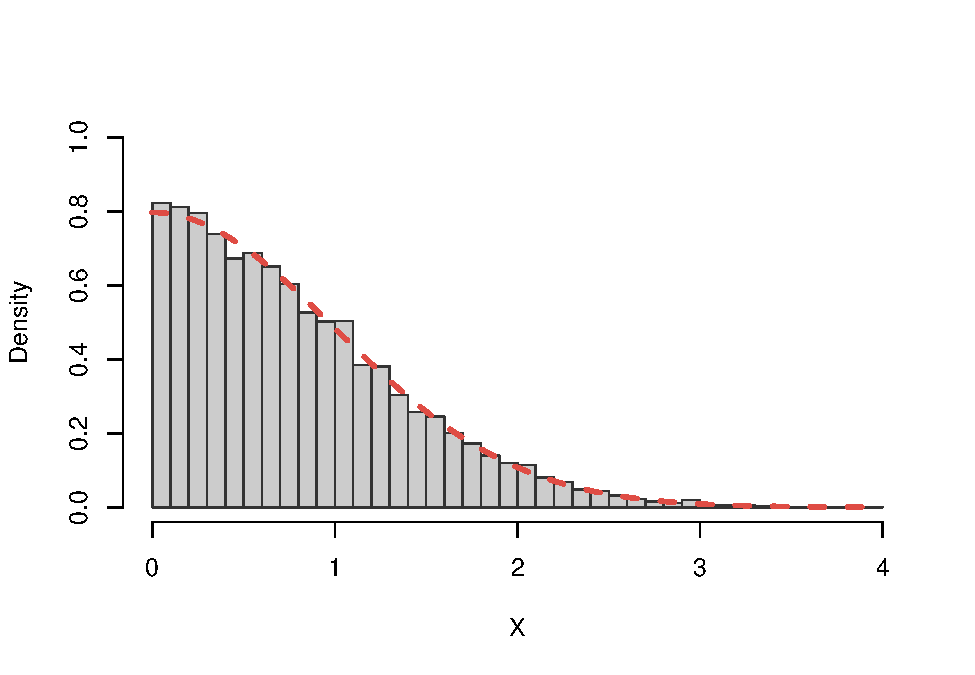
\includegraphics[width=0.8\linewidth]{Lab4_files/figure-latex/unnamed-chunk-35-1} \end{center}

\begin{rmdexercise}
Modificați codul de la exercițiul precedent pentru a simula un eșantion
dintr-o normală standard.
\end{rmdexercise}

Cum \(f\) (din problema 1) este densitatea unei normale standard
\(X\sim\mathcal{N}(0,1)\) condiționată la \(X>0\) și cum densitatea
normală este simetrică față de medie (0 în acest caz) algoritmul se
modifică acceptând \(x_n\) și \(-X_n\) cu probabilitatea de \(0.5\).

Astfel avem funcția:

\begin{Shaded}
\begin{Highlighting}[]
\NormalTok{f2 <-}\StringTok{ }\ControlFlowTok{function}\NormalTok{(x) \{}
  \KeywordTok{return}\NormalTok{(}\KeywordTok{dnorm}\NormalTok{(x,}\DecValTok{0}\NormalTok{,}\DecValTok{1}\NormalTok{))}
\NormalTok{\}}

\NormalTok{normal1 <-}\StringTok{ }\ControlFlowTok{function}\NormalTok{(n) \{}
\NormalTok{  res <-}\StringTok{ }\KeywordTok{numeric}\NormalTok{(}\DataTypeTok{length=}\NormalTok{n)}
\NormalTok{  i <-}\StringTok{ }\DecValTok{0}
  \ControlFlowTok{while}\NormalTok{ (i}\OperatorTok{<}\NormalTok{n) \{}
\NormalTok{    U <-}\StringTok{ }\KeywordTok{runif}\NormalTok{(}\DecValTok{1}\NormalTok{, }\DecValTok{0}\NormalTok{, }\DecValTok{1}\NormalTok{)}
\NormalTok{    X <-}\StringTok{ }\KeywordTok{rexp}\NormalTok{(}\DecValTok{1}\NormalTok{, }\DecValTok{1}\NormalTok{)}
    \ControlFlowTok{if}\NormalTok{ (c }\OperatorTok{*}\StringTok{ }\KeywordTok{g}\NormalTok{(X) }\OperatorTok{*}\StringTok{ }\NormalTok{U }\OperatorTok{<=}\StringTok{ }\KeywordTok{f}\NormalTok{(X)) \{}
\NormalTok{      i <-}\StringTok{ }\NormalTok{i}\OperatorTok{+}\DecValTok{1}
      
\NormalTok{      res[i] <-}\StringTok{ }\KeywordTok{ifelse}\NormalTok{(}\KeywordTok{runif}\NormalTok{(}\DecValTok{1}\NormalTok{) }\OperatorTok{<=}\StringTok{ }\FloatTok{0.5}\NormalTok{, X, }\OperatorTok{-}\NormalTok{X);}
\NormalTok{    \}}
\NormalTok{  \}}
  \KeywordTok{return}\NormalTok{(res)}
\NormalTok{\}}
\end{Highlighting}
\end{Shaded}

si testul

\begin{Shaded}
\begin{Highlighting}[]
\NormalTok{X <-}\StringTok{ }\KeywordTok{normal1}\NormalTok{(}\DecValTok{10000}\NormalTok{)}

\KeywordTok{hist}\NormalTok{(X, }\DataTypeTok{breaks=}\DecValTok{50}\NormalTok{, }
     \DataTypeTok{prob=}\OtherTok{TRUE}\NormalTok{, }
     \DataTypeTok{main=}\OtherTok{NULL}\NormalTok{, }
     \DataTypeTok{col=}\StringTok{"gray80"}\NormalTok{, }\DataTypeTok{border=}\StringTok{"gray20"}\NormalTok{)}

\KeywordTok{curve}\NormalTok{(f2, }\KeywordTok{min}\NormalTok{(X), }\KeywordTok{max}\NormalTok{(X), }\DataTypeTok{n=}\DecValTok{500}\NormalTok{,}\DataTypeTok{col =}\NormalTok{ myred, }\DataTypeTok{lty =} \DecValTok{2}\NormalTok{, }\DataTypeTok{lwd =} \DecValTok{3}\NormalTok{, }\DataTypeTok{add=}\OtherTok{TRUE}\NormalTok{)}
\end{Highlighting}
\end{Shaded}

\begin{center}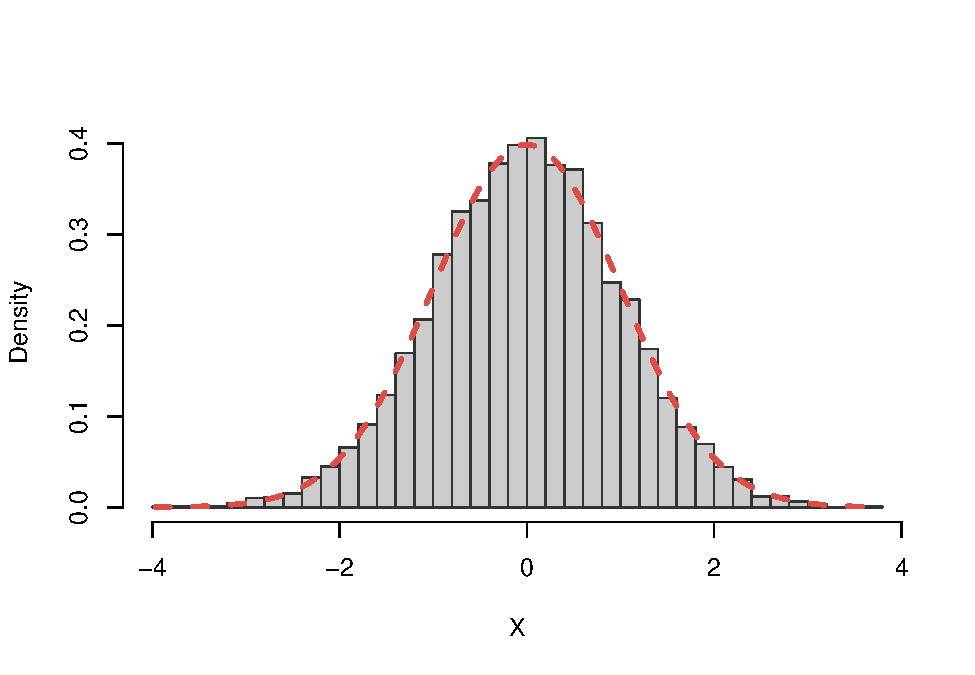
\includegraphics[width=0.8\linewidth]{Lab4_files/figure-latex/unnamed-chunk-38-1} \end{center}

\section{Simularea unei uniforme pe
disc}\label{simularea-unei-uniforme-pe-disc}

\begin{rmdexercise}
Considerăm pătratul \(C = [0,L]^2\) și discul \(D\) de centru
\((\frac{L}{2},\frac{L}{2})\) și rază \(\frac{L}{2}\). Considerăm șirul
de v.a. \(\left(Y_n\right)_{n\geq1}\) pe \(\mathbb{R}^2\) i.i.d.
repartizate uniform pe pătratul \(C\).

\begin{enumerate}
\def\labelenumi{\arabic{enumi}.}
\item
  Aproximați valoarea lui \(\pi\) prin ajutorul numărului de puncte
  \(Y_n\) care cad în interiorul discului \(D\) (Metoda respingerii)
\item
  Simulați \(n\) puncte uniforme pe disc.
\end{enumerate}
\end{rmdexercise}

\begin{enumerate}
\def\labelenumi{\arabic{enumi}.}
\tightlist
\item
  Definim v.a. \(X_n=\mathbf{1}_{\{Y_n\in D\}}\), \(n\geq1\), care
  formează un șir de v.a. i.i.d. de lege
  \(\mathcal{B}(\mathbb{P}(Y_n\in D))\), deoarece
  \(\left(Y_n\right)_{n\geq1}\) este un șir de v.a. i.i.d. repartizate
  uniform pe \(C\), \(\mathcal{U}(C)\). Din \emph{Legea Numerelor Mari}
  avem că
\end{enumerate}

\[
  \displaystyle\frac{1}{n}\sum_{i=1}^{n}X_{i} \overset{a.s.}{\to} \mathbb{E}[X_1] = \mathbb{P}(Y_1\in D),
\]

prin urmare trebuie să calculăm probabilitatea \(\mathbb{P}(Y_1\in D)\).
Știm că densitatea v.a. \(Y_1\) este dată de
\(f_{Y_1}(x,y)=\frac{1}{\mathcal{A}(C)}\mathbf{1}_{C}(x,y)\) de unde

\[
\begin{aligned}
  \mathbb{P}(Y_1\in D) &= \iint_{D}f_{Y_1}(x,y)\,dxdy = \iint \mathbf{1}_{D}(x,y)\mathbf{1}_{C}(x,y)\,dxdy\\
                       &= \frac{1}{\mathcal{A}(C)}\iint \mathbf{1}_{D}(x,y)\,dxdy = \frac{\mathcal{A}(D)}{\mathcal{A}(C)} = \frac{\pi \frac{L^2}{4}}{L^2} = \frac{\pi}{4}.
\end{aligned}
\]

Astfel, putem estima valoarea lui \(\pi\) prin
\(\displaystyle\frac{4}{n}\sum_{i=1}^{n}X_{i}\) pentru valori mari ale
lui \(n\).

\begin{Shaded}
\begin{Highlighting}[]
\CommentTok{# Estimam valoarea lui pi}

\NormalTok{L =}\StringTok{ }\DecValTok{3} \CommentTok{# lungimea laturii patratului }
\NormalTok{R =}\StringTok{ }\NormalTok{L}\OperatorTok{/}\DecValTok{2} \CommentTok{# raza cercului inscris}

\NormalTok{n =}\StringTok{ }\DecValTok{2000} \CommentTok{# numarul de puncte din patratul C}
\CommentTok{# generam puncte uniforme in C}
\NormalTok{x =}\StringTok{ }\NormalTok{L}\OperatorTok{*}\KeywordTok{runif}\NormalTok{(n)}
\NormalTok{y =}\StringTok{ }\NormalTok{L}\OperatorTok{*}\KeywordTok{runif}\NormalTok{(n)}

\CommentTok{# metoda respingerii (rejectiei)}
\NormalTok{l =}\StringTok{ }\NormalTok{(x}\OperatorTok{-}\NormalTok{R)}\OperatorTok{^}\DecValTok{2}\OperatorTok{+}\NormalTok{(y}\OperatorTok{-}\NormalTok{R)}\OperatorTok{^}\DecValTok{2} \CommentTok{# distanta dintre centrul cercului si punct}
\NormalTok{ind =}\StringTok{ }\NormalTok{l}\OperatorTok{<=}\NormalTok{(R)}\OperatorTok{^}\DecValTok{2} \CommentTok{# indicii pentru care distanta este mai mica sau egala cu R}

\NormalTok{xc =}\StringTok{ }\NormalTok{x[ind] }\CommentTok{# coordonatele punctelor din interiorul cercului  }
\NormalTok{yc =}\StringTok{ }\NormalTok{y[ind] }

\NormalTok{estimate_pi =}\StringTok{ }\DecValTok{4}\OperatorTok{*}\KeywordTok{sum}\NormalTok{(ind)}\OperatorTok{/}\NormalTok{n }\CommentTok{# estimarea lui pi}
\NormalTok{err =}\StringTok{ }\KeywordTok{abs}\NormalTok{(estimate_pi}\OperatorTok{-}\NormalTok{pi) }\CommentTok{# eroarea absoluta}
\end{Highlighting}
\end{Shaded}

Aplicând acest procedeu obținem că valoarea estimată a lui \(\pi\) prin
generarea a \(n=\) 2000 puncte este 3.162 iar eroarea absoluta este
0.02041.

\begin{enumerate}
\def\labelenumi{\arabic{enumi}.}
\setcounter{enumi}{1}
\tightlist
\item
  Una dintre metodele prin care putem simula puncte uniform repartizate
  pe suprafața discului \(D\) este \emph{Metoda respingerii}. Această
  metodă consistă în generarea de v.a. \(Y_n\) repartizate uniform pe
  suprafața pătratului \(C\), urmând ca apoi să testăm dacă \(Y_n\)
  aparține discului \(D\) (deoarece \(D\subset C\)). Dacă da, atunci le
  păstrăm dacă nu atunci mai generăm. Următoarea figură ilustrează
  această metodă:
\end{enumerate}

\begin{Shaded}
\begin{Highlighting}[]
\CommentTok{# figura }
\NormalTok{theta =}\StringTok{ }\KeywordTok{seq}\NormalTok{(}\DecValTok{0}\NormalTok{, }\DecValTok{2}\OperatorTok{*}\NormalTok{pi}\OperatorTok{+}\DecValTok{1}\NormalTok{, }\DataTypeTok{by =} \FloatTok{0.1}\NormalTok{)}
\NormalTok{xd =}\StringTok{ }\NormalTok{R}\OperatorTok{+}\NormalTok{R}\OperatorTok{*}\KeywordTok{cos}\NormalTok{(theta)}
\NormalTok{yd =}\StringTok{ }\NormalTok{R}\OperatorTok{+}\NormalTok{R}\OperatorTok{*}\KeywordTok{sin}\NormalTok{(theta)}

\KeywordTok{plot}\NormalTok{(x, y, }
     \DataTypeTok{col =} \StringTok{"grey80"}\NormalTok{, }\DataTypeTok{pch =} \DecValTok{16}\NormalTok{,}
     \DataTypeTok{asp =} \DecValTok{1}\NormalTok{, }
     \DataTypeTok{xlim =} \KeywordTok{c}\NormalTok{(}\DecValTok{0}\NormalTok{,}\DecValTok{3}\NormalTok{), }\DataTypeTok{ylim =} \KeywordTok{c}\NormalTok{(}\DecValTok{0}\NormalTok{,}\DecValTok{3}\NormalTok{),}
     \DataTypeTok{bty =} \StringTok{"n"}\NormalTok{)}

\KeywordTok{points}\NormalTok{(xc, yc, }\DataTypeTok{col =}\NormalTok{ myred, }\DataTypeTok{pch =} \DecValTok{16}\NormalTok{)}
\KeywordTok{lines}\NormalTok{(xd, yd, }\DataTypeTok{col =}\NormalTok{ myblue, }\DataTypeTok{lwd =} \DecValTok{3}\NormalTok{)}
\end{Highlighting}
\end{Shaded}

\begin{center}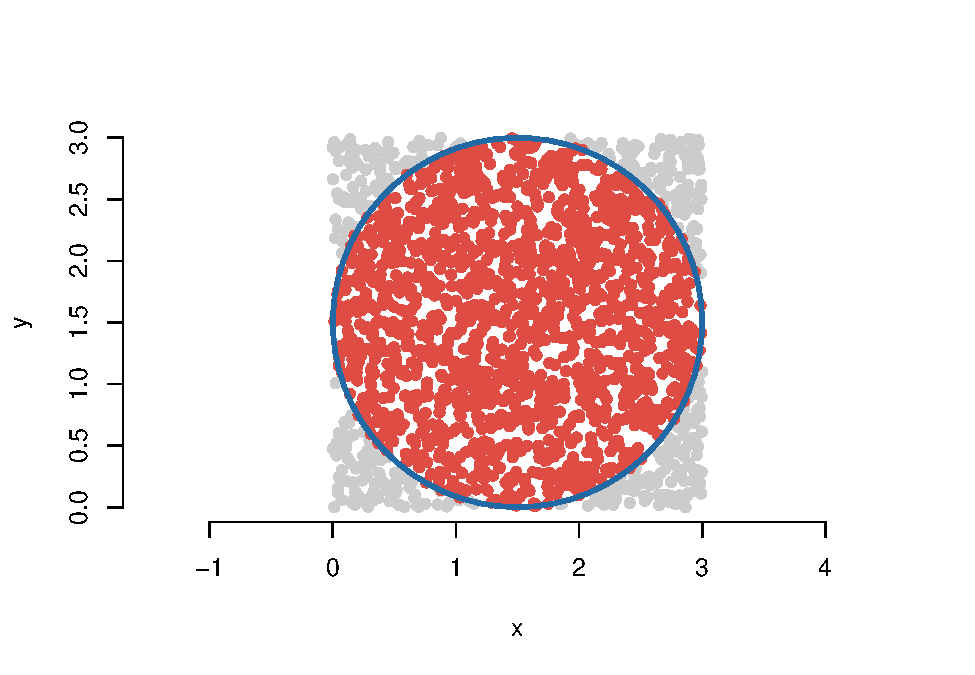
\includegraphics[width=0.8\linewidth]{Lab4_files/figure-latex/unnamed-chunk-41-1} \end{center}

Vom da mai jos o altă metodă de simulare a punctelor distribuite uniform
pe discul \(D\) de rază \(L\). O primă idee ar fi să generăm cuplul de
v.a. \((X_1,Y_1)\) așa încât \(X_1,Y_1\sim\mathcal{U}([0,L])\) și ele să
fie independente (ceea ce nu este adevărat în realitate). Vom vedea
(printr-o ilustrație grafică) că această abordare este greșită (punctele
sunt concentrate în centrul cercului).

O altă abordare este următoarea. Căutăm să simulăm un cuplu de v.a.
\((X,Y)\) care este uniform distribuit pe suprafața discului \(D\),
i.e.~densitatea cuplului este dată de
\(f_{(X,Y)}(x,y)=\frac{1}{\pi L^2}\mathbf{1}_{D}(x,y)\). Considerăm
schimbarea de variablile în coordonate polare: \(x=r\cos(\theta)\) și
\(y=r\sin(\theta)\). Obiectivul este de a găsi densitatea variabilelor
\(R\) și \(\Theta\).

Fie \(g(x,y)=\left(\sqrt{x^2+y^2},\arctan(y/x)\right)=(r,\theta)\),
transformarea pentru care avem \((R,\Theta)=g(X,Y)\). Știm că inversa
acestei transformări este
\(g^{-1}(r,\theta)=(r\cos(\theta),r\sin(\theta))\), prin urmare

\[
\begin{aligned}
  f_{(R,\Theta)}(r,\theta) &= f_{(X,Y)}\left(g^{-1}(r,\theta)\right)|\det(J_{g^{-1}}(r,\theta))|\\
                &= \frac{1}{\pi L^2}\mathbf{1}_{D}(r\cos(\theta),r\sin(\theta))\left|\begin{array}{cc}
                    \cos(\theta) & \sin(\theta)\\
                    r\sin(\theta) & -r\cos(\theta)
                \end{array}\right|\\
                &= \frac{1}{\pi L^2} \mathbf{1}_{[0,L]}(r)\mathbf{1}_{[0,2\pi]}(\theta)r.
\end{aligned}
\]

Observăm că densitatea (marginală) v.a. \(\Theta\) este

\[
\begin{aligned}
  f_{\Theta}(\theta) &= \int f_{(R,\Theta)}(r,\theta)\,dr = \mathbf{1}_{[0,2\pi]}(\theta)\int \frac{r}{\pi L^2} \mathbf{1}_{[0,L]}(r)\,d\theta\\
                     &= \frac{1}{\pi L^2} \mathbf{1}_{[0,2\pi]}(\theta) \frac{L^2}{2} = \frac{1}{2\pi} \mathbf{1}_{[0,2\pi]}(\theta),
\end{aligned}
\]

iar densitatea v.a. \(R\) este

\[
\begin{aligned}
  f_{R}(r) &= \int f_{(R,\Theta)}(r,\theta)\,d\theta = \frac{r}{\pi L^2} \mathbf{1}_{[0,L]}(r)\int_{0}^{2\pi}\,d\theta\\
                     &= \frac{r}{\pi L^2} \mathbf{1}_{[0,L]}(r)2\pi = \frac{2r}{L^2} \mathbf{1}_{[0,L]}(r).
\end{aligned}
\]

Din expresiile de mai sus putem observa că \(\Theta\) este o v.a.
repartizată uniform pe \([0,2\pi]\) și putem verifica ușor că legea v.a.
\(R\) este aceeași cu cea a v.a. \(L\sqrt{U}\) unde
\(U\sim\mathcal{U}([0,1])\).

Astfel pentru simularea unui punct \((X,Y)\) uniform pe \(D\) este
suficient să simulăm o v.a. \(\Theta\) uniform pe \([0,2\pi]\) și o v.a.
\(U\) uniformă pe \([0,1]\) și să luăm \(X=L\sqrt{U}\cos(\Theta)\) și
\(Y=L\sqrt{U}\sin(\Theta)\).

Următorul cod ne ilustrează cele două proceduri prezentate:

\begin{Shaded}
\begin{Highlighting}[]
\CommentTok{# rm(list=ls())}

\NormalTok{n =}\StringTok{ }\DecValTok{2000}\NormalTok{;}\CommentTok{# numarul de puncte}

\NormalTok{R =}\StringTok{ }\DecValTok{10}\NormalTok{;}\CommentTok{# raza cercului }

\NormalTok{theta =}\StringTok{ }\DecValTok{2}\OperatorTok{*}\NormalTok{pi}\OperatorTok{*}\KeywordTok{runif}\NormalTok{(n);}\CommentTok{# theta este uniforma pe [0,2*pi]}

\CommentTok{# versiunea gresita - r este uniforme pe [0,R]}
\NormalTok{r1 =}\StringTok{ }\NormalTok{R}\OperatorTok{*}\KeywordTok{runif}\NormalTok{(n);}

\NormalTok{x1 =}\StringTok{ }\NormalTok{r1}\OperatorTok{*}\KeywordTok{cos}\NormalTok{(theta);}\CommentTok{# coordonate polare}
\NormalTok{y1 =}\StringTok{ }\NormalTok{r1}\OperatorTok{*}\KeywordTok{sin}\NormalTok{(theta);}

\CommentTok{# versiunea corecta}
\NormalTok{r2 =}\StringTok{ }\NormalTok{R}\OperatorTok{*}\KeywordTok{sqrt}\NormalTok{(}\KeywordTok{runif}\NormalTok{(n));}

\NormalTok{x2 =}\StringTok{ }\NormalTok{r2}\OperatorTok{*}\KeywordTok{cos}\NormalTok{(theta);}\CommentTok{# coordonate polare}
\NormalTok{y2 =}\StringTok{ }\NormalTok{r2}\OperatorTok{*}\KeywordTok{sin}\NormalTok{(theta);}

\CommentTok{# schimbarea de variabila in coordonate polare: cercul}
\NormalTok{theta2 =}\StringTok{ }\KeywordTok{seq}\NormalTok{(}\DecValTok{0}\NormalTok{,}\DecValTok{2}\OperatorTok{*}\NormalTok{pi}\OperatorTok{+}\DecValTok{1}\NormalTok{,}\DataTypeTok{by=}\FloatTok{0.1}\NormalTok{) }
\NormalTok{xc =}\StringTok{ }\NormalTok{R}\OperatorTok{*}\KeywordTok{cos}\NormalTok{(theta2);}
\NormalTok{yc =}\StringTok{ }\NormalTok{R}\OperatorTok{*}\KeywordTok{sin}\NormalTok{(theta2);}

\CommentTok{# graficul}

\KeywordTok{par}\NormalTok{(}\DataTypeTok{mfrow =} \KeywordTok{c}\NormalTok{(}\DecValTok{1}\NormalTok{,}\DecValTok{2}\NormalTok{))}

\KeywordTok{plot}\NormalTok{(x1, y1,}
     \DataTypeTok{ylim =} \KeywordTok{c}\NormalTok{(}\OperatorTok{-}\DecValTok{11}\NormalTok{, }\DecValTok{11}\NormalTok{),}
     \DataTypeTok{col =}\NormalTok{ myred, }\DataTypeTok{pch =} \DecValTok{16}\NormalTok{,}
     \DataTypeTok{main =} \StringTok{"Versiunea gresita"}\NormalTok{, }\DataTypeTok{xlab =} \StringTok{"x"}\NormalTok{, }\DataTypeTok{ylab =} \StringTok{"y"}\NormalTok{, }\DataTypeTok{asp =} \DecValTok{1}\NormalTok{, }\DataTypeTok{bty =} \StringTok{"n"}\NormalTok{)}
\KeywordTok{lines}\NormalTok{(xc, yc, }\DataTypeTok{lwd =} \DecValTok{3}\NormalTok{, }\DataTypeTok{col =}\NormalTok{ myblue)}

\KeywordTok{plot}\NormalTok{(x2, y2,}
     \DataTypeTok{ylim =} \KeywordTok{c}\NormalTok{(}\OperatorTok{-}\DecValTok{11}\NormalTok{, }\DecValTok{11}\NormalTok{),}
     \DataTypeTok{col =}\NormalTok{ myred, }\DataTypeTok{pch =} \DecValTok{16}\NormalTok{,}
     \DataTypeTok{main =} \StringTok{"Versiunea corecta"}\NormalTok{, }\DataTypeTok{xlab =} \StringTok{"x"}\NormalTok{, }\DataTypeTok{ylab =} \StringTok{"y"}\NormalTok{, }\DataTypeTok{asp =} \DecValTok{1}\NormalTok{, }\DataTypeTok{bty =} \StringTok{"n"}\NormalTok{)}
\KeywordTok{lines}\NormalTok{(xc, yc, }\DataTypeTok{lwd =} \DecValTok{3}\NormalTok{, }\DataTypeTok{col =}\NormalTok{ myblue)}
\end{Highlighting}
\end{Shaded}

\begin{center}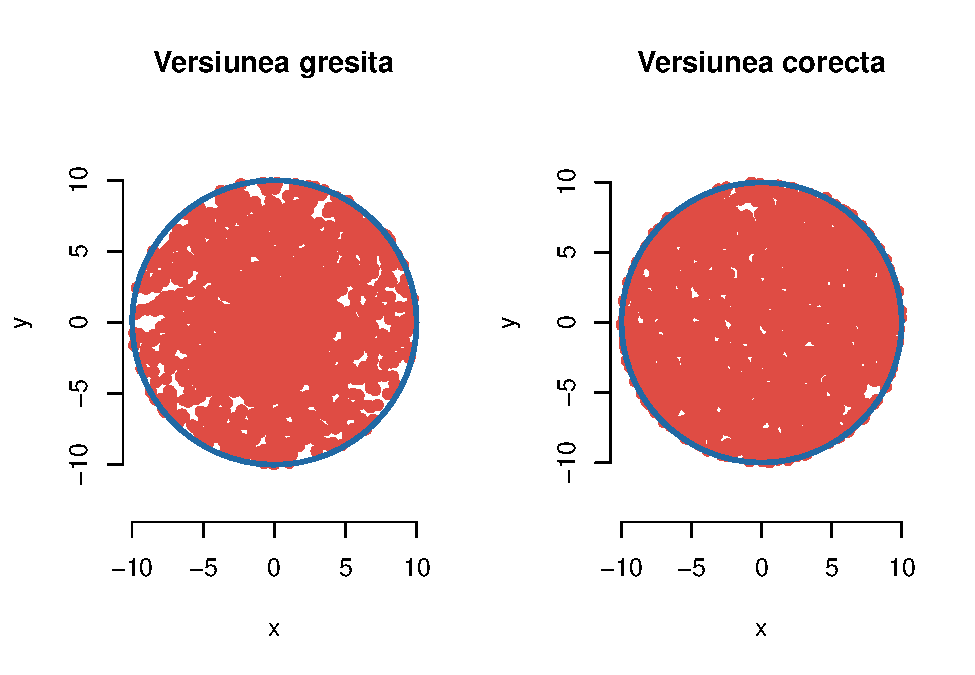
\includegraphics[width=0.8\linewidth]{Lab4_files/figure-latex/unnamed-chunk-42-1} \end{center}


\end{document}
